\documentclass[11pt,letterpaper]{article}
\usepackage[T1]{fontenc}
\usepackage{lmodern}
\usepackage[margin=0.94in,top=0.84in,bottom=0.88in,headheight=15pt,headsep=13pt]{geometry}
\usepackage{amsmath,amssymb,amsthm,mathtools,booktabs,tabularx,array}
\usepackage{microtype,xcolor,fancyhdr,titlesec,graphicx}
\usepackage{hyperref}
\definecolor{ink}{HTML}{173D49}
\definecolor{tone}{HTML}{365D68}
\hypersetup{colorlinks=true,linkcolor=tone,citecolor=tone,urlcolor=tone,pdftitle={The Mertens function in intuitionistic primitive recursive arithmetic},pdfauthor={Research report}}
\pagestyle{fancy}\fancyhf{}
\fancyhead[L]{\small\sffamily\color{tone}The Mertens function}
\fancyhead[R]{\small\sffamily\color{tone}Intuitionistic primitive recursive arithmetic}
\fancyfoot[R]{\small\sffamily\thepage}
\renewcommand{\headrulewidth}{0.3pt}
\titleformat{\section}{\Large\sffamily\bfseries\color{ink}}{\thesection}{0.6em}{}
\titleformat{\subsection}{\large\sffamily\bfseries\color{ink}}{\thesubsection}{0.55em}{}
\titlespacing*{\section}{0pt}{2.5ex plus .5ex minus .25ex}{1.0ex}
\titlespacing*{\subsection}{0pt}{1.8ex plus .4ex}{.5ex}
\newtheoremstyle{reportthm}{7pt}{6pt}{\itshape}{}{\bfseries\color{ink}}{.}{.5em}{}
\theoremstyle{reportthm}
\newtheorem{theorem}{Theorem}[section]
\newtheorem{lemma}[theorem]{Lemma}
\newtheorem{proposition}[theorem]{Proposition}
\newtheorem{corollary}[theorem]{Corollary}
\setlength{\parindent}{1.15em}
\setlength{\emergencystretch}{1.4em}
\setcounter{tocdepth}{1}
\raggedbottom
\newcommand{\proj}{https://github.com/VladimirReshetnikov/ProveIt/tree/65b76a5b8aa87ecad4103c2d287eff5660d3c84c/Logic/PrimitiveRecursiveArithmetic}
\begin{document}
\thispagestyle{plain}
{\noindent\sffamily\color{tone}\small NUMBER THEORY\quad / \quad CONSTRUCTIVE ARITHMETIC\par}
\vspace{1.3em}
{\noindent\sffamily\bfseries\color{ink}\fontsize{28}{32}\selectfont The Mertens function\par}
\vspace{.35em}
{\noindent\large\sffamily in intuitionistic primitive recursive arithmetic\par}
\vspace{.7em}
{\noindent\small 22 November 2026\par}
\vspace{1em}
\noindent The identity $\sum_{d\mid n}\mu(d)=[n=1]$ gives a short route from a bounded factorization algorithm to determinants, Farey sums and efficient evaluation of $M(N)$. It also gives the reciprocal zeta series. With explicit tail and contour bounds, we obtain symmetric Perron inversion, the squarefree-density constant, and $|M(N)|\le C_hN/(\log N)^h$ for every natural $h$, with primitive recursive constants. A separate argument recovers cancellation from ProveIt's effective prime number theorem. We prove an equivalence between the RH growth condition and quantitative zero exclusion on compact rectangles. A single certified zeta zero gives a bounded search for $|M(n)|>\sqrt n/32768$ beyond any starting point. Each assertion involving analysis has a finite-precision reading.

\vspace{.8em}
\noindent{\small\renewcommand{\arraystretch}{1.16}%
\begin{tabularx}{\linewidth}{@{}>{\raggedright\arraybackslash\bfseries}p{.21\linewidth}>{\raggedright\arraybackslash}Xr@{}}
\toprule
Area & Principal results & Sections\\ \midrule
Finite identities & Divisor inversion, totients, Chebyshev's $\psi$, hyperboloids, Redheffer determinant and Farey sums & \ref{sec:foundation}--\ref{sec:finite-representations}\\
Numerical results & Two algorithms and the maximum of $M(n)^2/n$ for $2\le n\le10\,000$ & \ref{sec:computing}\\
Analytic estimates & Dirichlet, Mellin and Perron formulas, squarefree density and unconditional cancellation & \ref{sec:analytic}--\ref{sec:cancellation}\\
Growth and zeros & Compact zero exclusion, square-root excursions and local residues & \ref{sec:growth}--\ref{sec:edges}\\
Formalization & Checked Lean theorems, definitions and proof obligations & \ref{sec:lean}\\
\bottomrule
\end{tabularx}}

\vspace{1em}
\noindent\textbf{Verification.} The accompanying Lean development checks general finite identities and the published 143-term initial table. The analytic arguments and the translation to first-order iPRA are human proofs and formalization plans. The reference programs give repeatable integer checks. The two requested articles supply the inventory of target statements \cite{wiki,mw}.

\vspace{1em}
\noindent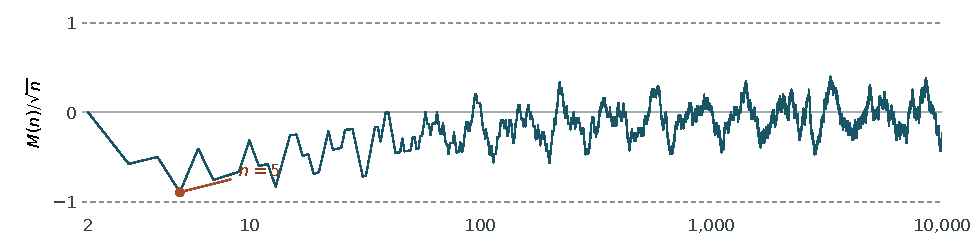
\includegraphics[width=\linewidth]{figures/mertens-quotient.pdf}
\par\noindent{\small\textbf{Mertens's original range.} The normalized sum at every integer from $2$ through $10\,000$, shown on a logarithmic horizontal scale. The largest absolute ratio is $2/\sqrt5$ at $n=5$.}
\newpage
\section{Arithmetic conventions and the basic cancellation}\label{sec:foundation}

We use first-order intuitionistic primitive recursive arithmetic (iPRA) as in ProveIt \cite{repo}. There is one numerical sort, a symbol and defining equations for each primitive recursive (PR) construction, and induction for quantifier-free formulas. Numerical parameters can be arbitrary. Bounded conjunction is a product of Boolean bits, bounded existence a finite disjunction with a least-index scan, and a bounded sum a primitive recursion. Thus correctness of all entries through $t$ may be an invariant for quantifier-free induction whenever entry correctness is given by a PR test. A loop with at most $b$ steps, including early termination, runs for $b$ ticks with a stopped flag. Products of signs, arrays, and permutations below all fall under these conventions.

For a concrete coding use $(u+v)^2+u$ for the pair $(u,v)$. The intervals from $s^2$ to $s^2+s$ are disjoint for distinct sums $s$, and the coordinates can be extracted by bounded search through the code. Iterated pairing with a length field codes lists. List traversal, updates and folding are PR by recursion on the stated length, with a fixed default for malformed codes. An integer may be a pair $(a,b)$ for $a-b$, with equality $a+d=b+c$ against $(c,d)$. Rationals add a positive denominator and use cross multiplication for order. All finite reindexings below are equalities of such sums, proved by distributivity and cutting a finite array into explicitly tested pieces. In particular signs can be decided for integers and rationals in intuitionistic logic.

\paragraph{Factorization with bounds.}
For $m\ge2$ take the least $d$ in $[2,m]$ dividing $m$. It is prime since a proper factor would be an earlier divisor. Divide out and repeat at most $m$ times, retaining the residual product as an invariant. The residual strictly decreases whenever it is above one, hence ends at one. To see uniqueness, the Euclidean algorithm terminates on a pair of naturals in at most the smaller input plus two division steps (positive divisors decrease). Back substitution supplies a signed B\'ezout identity. If $p$ is prime and $p\nmid a$, $\gcd(p,a)=1$, so $p\mid ab$ implies $p\mid b$ after multiplying that identity by $b$. Consequently the first prime in one factorization occurs in any other. Cancel it and iterate over the bounded lists. This proves existence and uniqueness with no unbounded minimization. For $m=1$ the list is empty.

Set $\mu(1)=1$. For $m\ge2$, set $\mu(m)=0$ if some prime square divides $m$, otherwise put $\mu(m)=(-1)^t$ for the number $t$ of prime factors. Define
\[
 M(0)=0,\qquad M(N)=\sum_{1\le m\le N}\mu(m).
\]
For a nonnegative rational $a/b$ with $b>0$ put $M(a/b)=M(\lfloor a/b\rfloor)$. For named real inputs the step-function value can be used when an integer part is given, or on a cell with certified endpoints. Identifying the integer part of a general Cauchy name at a jump would decide information unavailable at finite precision. Integrals of this particular step function will instead be defined by splitting at known integer endpoints.

\begin{lemma}[Cancellation of the divisor sum]\label{lem:cancel}
For $n\ge1$, $\displaystyle\sum_{d\mid n}\mu(d)=[n=1]$. This equation uniquely determines the values of $\mu$ on positive arguments.
\end{lemma}
\begin{proof}
At $1$ the sum is one. At $n>1$ let $p$ be its least prime factor. Each squarefree divisor not containing $p$ is paired with its product by $p$. The reverse map divides out $p$. The two signs are opposite, and the remaining divisors have weight zero. To prove uniqueness, write the equation as the value at $n$ in terms of proper divisors and use induction on equality of two candidate prefixes. Both changes of index are bounded by $n$.
\end{proof}

The graph has precise local structure. The jump at $n$ is $\mu(n)$, so the plateaus between consecutive sample values occur exactly at nonsquarefree arguments. Writing $E(N),O(N)$ for the two squarefree parity counts gives $M=E-O$, and the total variation through $N$ is $Q(N)=E+O=\sum_{n\le N}|\mu(n)|$. In particular
\[
 |M(v)-M(u)|\le v-u \quad(0\le u\le v),\qquad
 |M(N)|\le Q(N)\le N-\lfloor N/4\rfloor.
\]
Each multiple of $4$ has zero weight, which gives the last inequality. Since $M(2)=0$, the interval bound also gives $|M(N)|\le N-2$ for every $N\ge2$. The first inequality extends the source bound $|M(x)|\le x$ to intervals between integer arguments. If two integer values of $M$ straddle an integer level, the scan up to the later index finds an occurrence of the level because the first crossing has step size at most one. This is an effective discrete intermediate-value property.

\paragraph{What the analytic notation means.}
A real or complex number used below is given by rational approximations with certified errors, with a fixed PR program at each input schema. A comparison with a positive margin supplies a rational lower bound for it. Equality of two named quantities comprises the assertions at each demanded precision. For induction one fixes the final precision, bounds the finite computation and propagates rational error budgets. Section~\ref{sec:analytic} gives the elementary evaluators. The estimates in the subsequent proofs specify cutoff and mesh bounds. Numerical integrals and complex zeros enter only with the hypotheses and precision data stated for them.

\section{Exact identities from finite divisor sums}\label{sec:divisor-identities}
For $N\ge 0$ and $a\ge1$ put $q_N(a)=\lfloor N/a\rfloor$.
In particular $q_N(a)=0$ for $a>N$. Throughout this section the sums
with upper endpoint zero are empty and $M(0)=0$.

\begin{lemma}[Weighted floor sums]\label{lem:weightedsum}
For any finite integer table $w(1),\ldots,w(N)$,
\[
 \sum_{a=1}^{N} w(a)M(q_N(a))
 =\sum_{m=1}^{N}\sum_{d\mid m}\mu(d)w(m/d).
\]
\end{lemma}
\begin{proof}
Expand the left side as the sum of $w(a)\mu(d)$ over the positive pairs
with $ad\le N$. The map $(a,d)\longmapsto(ad,d)$ has inverse
$(m,d)\longmapsto(m/d,d)$ on the displayed divisor pairs. To implement
the change of order, enumerate $a,d,m\le N$ and insert the indicator
$[ad=m]$. Summing first over $m$ or first over $a$ gives the two
expressions. Finite double sums commute by induction on their side lengths.
\end{proof}

\begin{theorem}[Floor recurrence and quotient blocks]\label{thm:floor-recurrence}
For $N\ge1$,
\[
 \sum_{a=1}^{N}M(q_N(a))=1,\qquad
 M(N)=1-\sum_{a=2}^{N}M(q_N(a)).
\]
The recursion, together with $M(0)=0$, uniquely determines $M$.
\end{theorem}
\begin{proof}
Set $w(a)=1$ in Lemma~\ref{lem:weightedsum}. The divisor sum on the right
is $[m=1]$. The $a=1$ term on the left is $M(N)$ and all remaining
arguments are strictly smaller than $N$. If two candidate tables obey the
same equations through $N$, induction on the Boolean predicate that all
entries through $t$ agree gives equality through $N$.

For $1\le q\le N$, the indices $a$ giving quotient $q$ are exactly
\[
  q_N(q+1)<a\le q_N(q).
\]
Indeed $q\le N/a<q+1$ is equivalent to $a q\le N<a(q+1)$.
Thus a whole block in the sum carries the single value $M(q)$ with
multiplicity $q_N(q)-q_N(q+1)$, with the term $a=1$ removed when using
the recursion. If $u$ is the largest integer with $u^2\le N$, the
indices $a\le u$ yield at most $u$ quotients. For $a\ge u+1$, the
inequality $N<(u+1)^2$ gives $q_N(a)\le u$. There are at most $2u$
distinct positive quotients in total.
\end{proof}

\begin{theorem}[Totients and the second Chebyshev function]\label{thm:totient-chebyshev}
Let $\varphi(m)=\#\{1\le b\le m:\gcd(b,m)=1\}$, including
$\varphi(1)=1$. For $N\ge1$ one has
\begin{align*}
 \sum_{a=1}^N aM(q_N(a)) &= \sum_{m=1}^N\varphi(m),\\
 \sum_{a=1}^N M(q_N(a))\log a
     &= \sum_{\substack{p\ \mathrm{prime},\ j\ge1\\p^j\le N}}\log p
      =\psi(N).
\end{align*}
The second equality of functions admits an exact, integer-valued proof
for each prime coordinate of the logarithms.
\end{theorem}
\begin{proof}
The indicator of coprimality equals $\sum_{d\mid\gcd(b,m)}\mu(d)$.
For each $d\mid m$, precisely $m/d$ of the integers $1,\ldots,m$ are
multiples of $d$. Hence
$\varphi(m)=\sum_{d\mid m}\mu(d)(m/d)$, and the first formula follows
from Lemma~\ref{lem:weightedsum}.

Fix a prime $p\le N$. Write $v_p(a)$ for the largest $j\le a$ such that
$p^j\mid a$, for $a\ge1$. It equals the number of $j\ge1$ such that
$p^j\mid a$. Set $w(a)=v_p(a)$ in the lemma. For each $m$ the inner sum is
\[
 \sum_{d\mid m}\mu(d)v_p(m/d)
 =\sum_{\substack{j\ge1\\p^j\mid m}}\;\sum_{d\mid m/p^j}\mu(d)
 =[m=p^j\text{ for some }j\ge1].
\]
Indeed the inner divisor sum vanishes unless $p^j=m$, and then it is
one. Consequently the coefficient of the formal symbol $\log p$ on each
side of the Chebyshev formula is $\#\{j\ge1:p^j\le N\}$. Unique
factorization gives $\log a=\sum_{p\le N}v_p(a)\log p$ in these
coordinates. Substituting the usual logarithms in this finite identity
gives the displayed formula. Its multiplicative form in positive rationals is
\[
  \prod_{a=1}^N a^{M(q_N(a))}=\operatorname{lcm}(1,\ldots,N),
\]
since the exponent on the right is the largest $j$ with $p^j\le N$,
which equals the same count. Move negative powers to the other side to
obtain a natural-number equality. The prime and exponent tests have
bounds $p,j\le N$.
\end{proof}

\subsection{Ordered products beneath a hyperboloid}
Let $H_k(N)$ count ordered $k$-tuples $(a_1,\ldots,a_k)$ of integers
at least two satisfying $a_1\cdots a_k\le N$. For $N\ge1$ the empty
tuple gives $H_0(N)=1$. Write $L_N$ for the largest $k\le N$ with
$2^k\le N$.

\begin{theorem}[Finite hyperboloid expansion]\label{thm:hyperboloid}
For $N\ge1$,
\[
 M(N)=\sum_{k=0}^{L_N}(-1)^k H_k(N).
\]
For $N\ge2$, the first two terms are $1-(N-1)$.
\end{theorem}
\begin{proof}
On tables indexed by $1,\ldots,N$, let
$(Tg)(t)=\sum_{a=2}^{t}g(q_t(a))$. For these $a$ the quotient is at
least one. The floor recurrence reads $M=\mathbf{1}-TM$, where
$\mathbf{1}$ is the constant table of ones. Repeated substitution and
the additivity of $T$ give, for every $s\ge0$,
\[
 M=\sum_{k=0}^s(-1)^kT^k\mathbf{1}+(-1)^{s+1}T^{s+1}M.
\]
This follows by induction starting with the floor recurrence. For every
positive $a,b$ one has $q_{q_t(a)}(b)=q_t(ab)$ since for any $j$ both
quotients are at least $j$ exactly when $jab\le t$.
Induction on $k$ now identifies $(T^kg)(t)$ with the sum over tuples
counted by $H_k(t)$ of $g(\lfloor t/(a_1\cdots a_k)\rfloor)$. Cutting
off or prepending the first factor gives the two inverse enumerations
in the induction step. Taking $s=L_N$ kills the last table since
every tuple with $L_N+1$ factors has product at least $2^{L_N+1}>N$.
Taking $g=\mathbf{1}$ proves the formula. Tuple codes are bounded by
$(N+1)^k$ using base $N+1$. Alternatively $H_{k+1}=TH_k$ computes all
needed counts using bounded tables.
\end{proof}

\section{Two finite representations of \texorpdfstring{$M(N)$}{M(N)}}\label{sec:finite-representations}
\subsection{The Redheffer determinant}
For $N\ge1$, the Redheffer matrix $R$ has indices $1\le i,j\le N$ and entries
\[
 R_{ij}=[j=1\ \text{or}\ i\mid j].
\]
\begin{theorem}\label{thm:redheffer}
$\det R=M(N)$.
\end{theorem}
\begin{proof}
Use the integer Leibniz determinant, the sum over permutations $\sigma$
of $(-1)^{\operatorname{inv}(\sigma)}\prod_i R_{i,\sigma(i)}$, where
$\operatorname{inv}$ counts inversions. Replace the first row by
$\sum_{i=1}^N\mu(i)R_{i,*}$. Multilinearity in this row follows by
distributing the product in each permutation term. For $i>1$, replacing
row 1 by row $i$ gives determinant zero. To see this, pair the term of
$\sigma$ with the term in which its images at positions $1$ and $i$
are exchanged. Their products agree. The exchange is a composition of
$2(i-1)-1$ adjacent exchanges, each of which changes inversion parity.
This explicitly pairs opposite signs. Since $\mu(1)=1$, the row
replacement preserves the determinant.

The new first entry is $M(N)$ since the first column consists of ones.
For $j>1$ the new entry is $\sum_{i\mid j}\mu(i)=0$. A possibly
nonzero permutation term therefore has $\sigma(1)=1$. For $i\ge2$ it
must have $i\mid\sigma(i)$ and thus $i\le\sigma(i)$. The sum of all
images equals the sum of the indices. It follows that $i=\sigma(i)$ at
every position, since any strict inequality would increase the sum. Only
the identity term can contribute. Its value is $M(N)$. All the entries,
permutations and inversion tests are finite. One may enumerate $N$-digit
base-$(N+1)$ codes, retaining just the lists containing each symbol
$1,\ldots,N$ exactly once.
\end{proof}

\subsection{The Farey sum and all its integer frequencies}
For $N\ge1$, let $\mathcal F_N$ consist of $0/1$ and all fractions
$a/q$ with $1\le a\le q\le N$ and $\gcd(a,q)=1$. This lists $1/1$
exactly once. Reduced representations are unique by cross multiplication
and prime factorization. The order of the list will not affect its sum.

\begin{theorem}[Farey and Ramanujan sums]\label{thm:farey}
For every $h\ge0$,
\begin{align*}
 c_q(h)&:=\sum_{\substack{1\le a\le q\\\gcd(a,q)=1}}
       e^{2\pi i ha/q}=\sum_{r\mid\gcd(q,h)}r\mu(q/r),\\
 \sum_{x\in\mathcal F_N} e^{2\pi i h x}
    &= 1+\sum_{\substack{1\le r\le N\\r\mid h}}rM(q_N(r)).
\end{align*}
Thus $M(N)=-1+\sum_{x\in\mathcal F_N}e^{2\pi i x}$ and
$|\mathcal F_N|=1+\sum_{m\le N}\varphi(m)$, where $m$ starts at one.
The finite arithmetic interpretation of the exponentials is made explicit below.
\end{theorem}
\begin{proof}
Expand the indicator of $\gcd(a,q)=1$ as $\sum_{d\mid\gcd(a,q)}\mu(d)$.
For a fixed $d\mid q$ write $a=db$, $r=q/d$. Its contribution is
$\mu(d)\sum_{b=1}^r e^{2\pi i hb/r}$, a sum around a regular polygon.
If $r\mid h$, this last sum is $r$. Otherwise put $z=e^{2\pi i h/r}$.
Multiplication of $z+\cdots+z^r$ by $1-z$ gives $z(1-z^r)=0$, and
$z\ne1$. Hence the sum is zero. This proves the formula for $c_q(h)$.
Add the extra term $1$ from $0/1$ and sum over $q\le N$. For each
$r\mid h$ write $q=rt$. The inner sum over $t\le q_N(r)$ is $M(q_N(r))$,
which gives the claimed expression. At $h=1$ only $r=1$ survives. At
$h=0$ every positive $r$ divides $h$, so Theorem~\ref{thm:totient-chebyshev}
gives the cardinality.

Here is an integer-polynomial certificate for the polygon calculation.
It makes the preceding complex notation disposable. Put $L=N!$, and work
in the ring of length-$L$ integer coefficient lists with cyclic convolution,
written $\mathbb Z[X]/(X^L-1)$. Multiplication by $X^j$ rotates a list
by $j\bmod L$. Encode the first displayed sum by the polynomial
\[
 C_{q,h}(X)=\sum_{\substack{1\le a\le q\\\gcd(a,q)=1}}
    X^{(ha(L/q)\bmod L)},\qquad
 D_L(X)=\prod_{k=1}^{L-1}(1-X^k).
\]
For $q\le N$ one has the exact coefficientwise equality
\[
 D_L C_{q,h}=D_L\sum_{r\mid\gcd(q,h)}r\mu(q/r)
       \pmod{X^L-1}.
\]
To verify it, perform the same divisor-indicator expansion. In a block
of length $r$, put $k=h(L/r)\bmod L$. If $r\mid h$, then $k=0$ and the
block is $r$. Otherwise $1\le k<L$. For the block
$G=X^k+\cdots+X^{rk}$ the telescoping equality
$(1-X^k)G=X^k(1-X^{rk})=0$ holds in the cyclic lists because $L\mid rk$.
The factor $1-X^k$ occurs in $D_L$, so $D_L G=0$. This proves the
certificate using bounded coefficient arithmetic, including $L=1$, when
the product is empty. In the usual complex interpretation put
$X=e^{2\pi i/L}$. Its order is $L$, hence every factor of $D_L(X)$ is
separated from zero. Indeed for $1\le k<L$ put $b=\min(k,L-k)$.
Then $|1-X^k|=2\sin(\pi b/L)\ge2\pi/(3L)\ge1/L$, using the elementary
sine estimate on $[0,\pi/2]$ proved in Section~\ref{sec:squarefree}.
Thus cancellation gives the stated complex identity. Cancellation of
$D_L$ requires this evaluation or the primitive-root ring below. All induction in
the certificate ranges over finite coefficient vectors, divisor lists or
products with displayed bounds.
\end{proof}

The same certificate gives equality inside an explicit ring representing a
primitive root, entirely in arithmetic. Here are the construction and the
reason cancellation works there. Write $B_m=X^m-1$ and proceed in increasing
order $1\le m\le L$. Define $P_m$ by monic polynomial division from
\[
 B_m=P_m\prod_{d\mid m,\ d<m}P_d.
\]
We verify simultaneously over $\mathbb Q[X]$ that each division is exact
and that all polynomials obtained are pairwise coprime. A previous
$P_d$ with $d\mid m$ divides $B_d$ and hence $B_m$. The previous factors
are pairwise coprime, so their product divides $B_m$ by the polynomial
B\'ezout identity applied successively. Monic long division also gives
integer coefficients for the quotient. If $e\mid m$ and $e<m$, a common
nonconstant factor of $P_m,P_e$ would give a square dividing $B_m$,
impossible since $B_m$ is coprime to its derivative $mX^{m-1}$.
For $e<m$ with $e\nmid m$, put $g=\gcd(e,m)<e$. Reduction of the larger
exponent modulo the smaller in the Euclidean algorithm gives
$\gcd(B_e,B_m)=B_g$. But $B_g=\prod_{d\mid g}P_d$ is coprime to $P_e$
by the induction hypothesis, which excludes a common factor of $P_e,P_m$.
This completes the simultaneous induction.

Taking degrees gives $\sum_{d\mid m}\deg P_d=m$. Grouping the fractions
$a/m$ for $1\le a\le m$ by their reduced denominators gives
$\sum_{d\mid m}\varphi(d)=m$. Subtraction of the proper-divisor terms,
in increasing order of $m$, now yields $\deg P_m=\varphi(m)\ge1$.
The ring of rational lists representing remainders modulo $P_L$ therefore
contains the rational constants faithfully. The class of $X$ satisfies
$X^L=1$. For $1\le k<L$, put $g=\gcd(k,L)<L$. Any common divisor of
$P_L$ and $X^k-1$ divides $B_g$, and $P_L$ is coprime to every $P_d$
with $d\mid g$. Thus $1-X^k$ has a B\'ezout inverse modulo $P_L$. Reducing
the cyclic-list certificate modulo $P_L$ and multiplying by these inverses
gives $C_{q,h}=c_q(h)$, with $c_q(h)$ the integer divisor sum, in this
ring. All polynomial divisions with remainder and extended Euclidean
algorithms here use bounded fuel because a nonzero division step lowers the
current degree, and a Euclidean step lowers the divisor degree. Tables
of previously constructed polynomials, rational coefficients, and
B\'ezout coefficients can be carried through these primitive recursions.
The induction on $m$ checks coprimality by computing monic gcds for all
indices up to $m$.

\section{Algorithms and the numerical claims}\label{sec:computing}

\begin{theorem}[All values and an isolated value]\label{thm:algorithm}
All the values through $N$ take $O(N)$ word operations and $O(N)$ words. For one value at $N\ge1$, the quotient recurrence takes $O(N^{2/3})$ word operations and $O(N^{2/3})$ words with the cutoff below.
\end{theorem}
\begin{proof}
For the table maintain a list of the primes found and a Boolean composite array initialized to false. Set $\mu(1)=1$. In increasing order of $i\ge2$, if $i$ is unmarked append it to the prime list and set $\mu(i)=-1$. For each prime $p$ in list order form $j=ip$. Stop if $j>N$. Mark $j$ composite. If $p\mid i$, set $\mu(j)=0$ and end this inner loop. Otherwise set $\mu(j)=-\mu(i)$ and continue.

Every composite $j$ has the unique generating pair $(i,p)$ with $p$ its least prime factor and $i=j/p$. Its least factor satisfies $p\le i$, and no prime below $p$ divides $i$. The pass at $i$ therefore reaches $p$. Conversely each product generated has $p$ as least factor, by the stopping condition. Thus the prime test on an unmarked $i$ is justified inductively, each composite is marked just once, and the update for $\mu$ follows from its prime exponents. There is at most one extra terminating test per outer iteration. A final prefix sum gives $M$.

For the isolated-value method let $b=\lceil\sqrt[3]N\rceil$, $y=\min(N,b^2)$ and $K=\lfloor N/(y+1)\rfloor\le b$. First sieve to $y$. For $i=K,K-1,\ldots,1$ compute the value at $v=\lfloor N/i\rfloor$. In its recurrence, starting at $a=2$, one whole quotient block has
\[
 u=\lfloor v/a\rfloor,\qquad e=\lfloor v/u\rfloor,\qquad
 \text{contribution }(e-a+1)M(u).
\]
Advance to $e+1$. For $u\le y$ use the sieve. For $u>y$, use the previously computed entry at index $ia$, since $u=\lfloor N/(ia)\rfloor$ and $i<ia\le K$. This proves the reverse-loop invariant and correctness, including the case $K=0$ when the sieve already gives the answer.

There are at most $2\lfloor\sqrt{N/i}\rfloor$ blocks at $i$. To sum this bound count the pairs $(i,j)$ with $1\le i\le K$, $j\ge1$ and $ij^2\le N$. Those with $j\le b$ contribute at most $b^2$ and the others at most $\sum_{j>b}N/(j(j-1))=N/b\le b^2$. This proves the time bound with integer cutoffs throughout. A running total in a recurrence has magnitude at most $1+N^2$. Indices and products fit in a constant multiple of $\log(2N)$ bits. The operation model allows indexed word reads and writes and integer division. With schoolbook word arithmetic in a random-access bit-cost model one can charge $O(\log^2(2N))$ per operation, giving the $O_\varepsilon(N^{2/3+\varepsilon})$ exponent. The operation-count claim concerns this algorithm. Other methods achieve smaller space bounds \cite{ht}.
\end{proof}

\paragraph{An independent formula for verification.}
Let $r=\lfloor\sqrt N\rfloor$. Using $\mu*\mu*\mathbf1=\mu$, sum the triple convolution over $abc\le N$ with weight $\mu(a)\mu(b)$. The regions $a>r$ and $b>r$ are disjoint. For fixed $a>r$ the sum on $(b,c)$ is $\sum_{m\le N/a}\sum_{b\mid m}\mu(b)=1$. Thus these two regions together contribute $2(M(N)-M(r))$. Summing $c$ in the remaining region and rearranging gives the identity used in the second computation \cite{ht}:
\[
 M(N)=2M(r)-\sum_{a,b\le r}\mu(a)\mu(b)\left\lfloor\frac{N}{ab}\right\rfloor.
\]

\paragraph{Exact finite evaluations.}
Both isolated-value algorithms yield the following ten integers.
\begin{center}
\begin{tabular}{@{}lrrrrrrrrrr@{}}
\toprule
$j$&0&1&2&3&4&5&6&7&8&9\\
$M(10^j)$&1&$-1$&1&2&$-23$&$-48$&212&1037&1928&$-222$\\
\bottomrule
\end{tabular}
\end{center}
For $N=1,\ldots,12$ the values are
$1,0,-1,-1,-2,-1,-2,-2,-2,-1,-2,-2$. The first ten positive zero arguments are
$2,39,40,58,65,93,101,145,149,150$. The full table to $428$ recovers the displayed initial $143$ terms, the displayed zero sequence, and the seven level sets in the two articles over their displayed ranges. The per-integer table is in \texttt{verification/initial-values.csv}. The program lists all the level hits over the required interval.

More sharply, on the integers $2\le n\le10\,000$ the maximum of $M(n)^2/n$ is $4/5$, first attained at $5$. The program verifies this by comparing integer cross products using two independent definitions of $\mu$. It uses the sieve and independently performs the update $\mu(m)\mathrel{-}=\mu(d)$ on each proper multiple $m$ of successive $d$, starting from the array $\delta$. Before visiting $d$, all contributions of its proper divisors have already been subtracted. This proves the update by the divisor identity. On each cell $[n,n+1)$ the largest ratio $M(n)^2/x$ occurs at $n$. On $(1,2)$ it is $1/x<1$. Together these give Mertens's historical strict inequality on $1<x\le10\,000$. For each finite calculation the proof rule in iPRA is evaluation of closed PR terms by their defining equations. The bundled scripts are reproducible evaluations, with the mathematical justifications above.

\paragraph{The disproof as a logical statement.}
The 1985 result of Odlyzko and te Riele gives excursions on both sides of the square-root bounds \cite{ot}. Its strict-excess conclusion implies $\exists n>1\ [M(n)^2>n]$ by taking an integer part. At the metamathematical level every true closed existential statement with a PR witness test has an iPRA proof obtained by evaluation at a witnessing numeral followed by existential introduction. This observation identifies the proof-theoretic status of the individual existential statement. It supplies neither that numeral nor a uniform oscillation theorem. The large oscillations in the 1985 paper and the effective bound of Pintz quoted in \cite{ht} remain external inputs here.

\section{The zeta identities with error bounds}\label{sec:analytic}

The analytic variable can be kept outside the language of iPRA. A rational
complex approximation is a pair of rational numbers. A name for a number
supplies primitive recursive approximants within $2^{-j}$ at precision $j$.
A statement about arbitrary such inputs is a schema in these names, or a
finite calculation with input approximations and their error bounds. In
particular, no evaluator for arbitrary primitive recursive programs is
needed inside arithmetic. Equality of named quantities means agreement at
every precision, with errors included. Throughout this section assume a
supplied integer $q\ge1$ with $\sigma=\operatorname{Re}s\ge1+1/q$
and a supplied integer upper bound on $|s|$. Both are quantitative
inputs to the estimates.

\paragraph{Elementary analytic operations.}
Here are details of the rational interpretation used below. For positive
rational $u$, write $u=2^jv$, $1\le v<2$, by bounded doubling of the
numerator or denominator. Compute $\log u=j\log 2+\log v$ using
\[
   \log v=2\sum_{h=0}^{K-1}\frac{w^{2h+1}}{2h+1}+E_K,
   \qquad w=\frac{v-1}{v+1},\qquad
   |E_K|\le \frac{2|w|^{2K+1}}{1-|w|^2}.
\]
Use the same formula at $v=2$. It follows by summing the finite geometric
identity for $1/(1-w^2)$ and integrating. For $|z|\le B$ with integral
$B\ge1$, the exponential Taylor series beyond index $2B$ has successive
absolute terms in ratio at most $1/2$. The term at $2B$ is at most
$B^{2B}$, so another $2B^2+j+4$ terms give error below $2^{-j}$.
Thus $x^{-s}=\exp(-s\log x)$ for positive $x$ has an explicit
rational algorithm, also for named $x$ on an interval bounded away from
zero. The formulae $(\log x)'=1/x$, $(e^z)'=e^z$, the exponential
addition law, and $|e^{u+iv}|=e^u$ follow by the same geometric
remainders for the differentiated series, the binomial formula for their
product, and $e^{iv}e^{-iv}=1$. For real arguments one may equivalently
define $\log$ by integration of $1/x$. Differentiating
$e^{\log x}/x$ shows it is constant and evaluation at $1$ gives its
value. In these uses the fundamental theorem of calculus has a finite
proof by subdivision. On an interval of length $L$ where $|F''|\le B$, summing
the first-order increments of $F$ over a mesh of width $h$ gives
a left sum for $F'$ with error at most $BLh$.
For the displayed series the increment estimate itself follows by the
binomial formula on polynomials followed by the tail bounds on the
first two derivatives. The product and quotient rules preserve the
estimate, with a positive lower bound for each denominator. Oscillatory
factors will only be integrated on bounded intervals at a time. On
each segment all these derivative bounds are obtained by replacing
the arguments by their supplied upper bounds, and replacing $e^B$ by
$3^{\lceil B\rceil}$ for $B\ge0$. This provides a primitive recursive
mesh at any requested precision. For a finite chain of $H$ arithmetic
operations on approximations, with all magnitudes bounded by $A\ge2$
and every divisor bounded below in absolute value by $1/A$, requesting
input errors $\le 2^{-j}(8A^3)^{-H-1}$ suffices for final error
$2^{-j}$. Indeed addition, multiplication, and division amplify the
larger of the two operand errors by at most $8A^3$ while the divisor
error stays below $1/(2A)$. Induction on the rational error inequality
implements the chain for variable $H$.

\begin{theorem}[Reciprocal Dirichlet series and prime product]
For the indicated $s$ let
\[
 Z_N(s)=\sum_{n=1}^N n^{-s},\qquad
 D_N(s)=\sum_{n=1}^N\mu(n)n^{-s},\qquad
 P_N(s)=\prod_{p\le N,\ p\ \mathrm{prime}}(1-p^{-s}).
\]
Then $Z_N$ names $\zeta(s)$, and $D_N$ and $P_N$ both name
$1/\zeta(s)$. Uniform tail estimates are available given the same $q$.
\end{theorem}
\begin{proof}
On the block $2^j\le n<2^{j+1}$ the sum of $n^{-\sigma}$ is at
most $2^{-j/q}$. Group the blocks in lots of $q$. Every finite tail
starting at $n\ge2^{qk}$ has absolute majorant $2q\,2^{-k}$,
and the full sum has majorant $2q$. For $N\ge2^{2qk}$ multiply
the two finite sums $Z_N D_N$. Terms with $ab\le N$ sum to $1$ by
$\sum_{d\mid m}\mu(d)=[m=1]$. Every remaining pair has
$a>\sqrt N$ or $b>\sqrt N$. Dropping signs and extending each
rectangle of summation gives
\[
                 |Z_N D_N-1|\le 8q^2 2^{-k}.
\]
Consequently the product of the two names is $1$. In particular, the
absolute bound $2q$ on the second factor separates the first factor
from zero by $1/(2q)$. Expanding $P_N$ chooses subsets of the primes
up to $N$. The signed monomial attached to a subset with product $m$
is $\mu(m)m^{-s}$. Unique factorization gives distinct products,
and every squarefree $m\le N$ occurs. The discrepancy from $D_N$
is bounded by the absolute tail after $N$, even though the largest
product can be as large as $N!$. This proves the three assertions.
\end{proof}

\begin{theorem}[Mellin formula and its finite version]
For $N\ge1$,
\[
 s\int_1^{N} M(\lfloor t\rfloor)t^{-s-1}\,dt
      =D_N(s)-M(N)N^{-s}.
\]
Its limit is $1/\zeta(s)$. At $N\ge2^{qk}$ the error from the
limiting value is at most $(2q+1)2^{-k}$.
\end{theorem}
\begin{proof}
On $[m,m+1]$ use the endpoint difference $m^{-s}-(m+1)^{-s}$ as
the integral of $s t^{-s-1}$. Isolated endpoint values have zero
contribution, as is witnessed by meshes of arbitrarily small width.
After multiplication by $M(m)$ and summation for $1\le m<N$, the
successive differences of $M$ are $\mu$, yielding the displayed
identity, also at $N=1$. The boundary term has absolute value at most
$N^{1-\sigma}\le2^{-k}$. The Dirichlet tail gives the remaining
error. The absolute integral beyond $N$ is bounded by
$|s|\int_N^\infty t^{-\sigma}dt\le q|s|N^{-1/q}$, as follows by
integrating a power over finite intervals. This also permits arbitrary
upper endpoints in the limit.
\end{proof}

\subsection{Perron inversion and the value at a jump}

Take $x=a/b>0$ rational, with $a,b$ positive integers. Define
$M_0(x)=M(\lfloor x\rfloor)$ when $x$ is nonintegral, and
$M_0(m)=M(m)-\mu(m)/2$ at a positive integer $m$. At $m$, twice
this value is $M(m-1)+M(m)$. This distinction affects the integral
displayed in the Wikipedia article even at $x=1$.

\begin{theorem}[Symmetric Perron inversion]\label{thm:perron}
For $c\ge1+1/q$ real, let $X$ be an integer bound on
$\max(1,x^c)$, for example $X=\max(1,a)^{\lceil c\rceil}$ when
$c$ is rational (a supplied integer upper bound for $c$ suffices).
For every integer $T\ge2c$,
\[
 \left|\frac{1}{2\pi i}\int_{c-iT}^{c+iT}
       \frac{x^s}{s\zeta(s)}\,ds-M_0(x)\right|
 \le \frac{6qX(a+1)+c}{T}.
\]
In particular the normalized integral has a primitive recursive
convergence modulus. The same conclusion holds on named inputs
given a known floor and positive separation from the adjacent integers,
with the corresponding lower bound on $|\log(x/n)|$.
\end{theorem}
\begin{proof}
Put $y=\log(x/n)$ and write $K_T(y)$ for the normalized integral
of $e^{ys}/s$ along this vertical segment. When $y>0$ close the
rectangle with the left edge at $c-T$, traversing it counterclockwise.
When $y<0$ close on the right at $c+T$. The normalized integral on
the closed rectangle is respectively $1$ or $0$. To verify this
directly, subtract $1/s$ from the integrand. The remainder has
primitive
\[
           \sum_{j\ge1} \frac{y^j s^j}{j\,j!}.
\]
Its convergence and the convergence of its differentiated series on
the rectangle follow from the exponential tail estimate, so endpoint
differences cancel on the four sides. For $ds/s$ the real part is
$d\log|s|$. The imaginary part is the increment of the angle.
Explicitly in a right or left half-plane chart this differential is
$d\arctan(v/u)$ for $s=u+iv$, and in a top or bottom chart it is
$-d\arctan(u/v)$. Subdivide edges at the axes and use the continuous
angle in each quadrant. Adjacent angle values agree at the axes on
the same turn. A contour wholly in the right half-plane lies in one
chart and the endpoint increments telescope to zero. A
counterclockwise rectangle surrounding $0$ runs once through the
four successive axis directions, which advances the angle by
$4(\pi/2)=2\pi$. These chart computations are rationally effective:
$\arctan t=\int_0^t(1+u^2)^{-1}du$ and $\pi=4\arctan 1$.
The quarter-turn convention follows from
$\arctan t+\arctan(1/t)=2\arctan 1$ for $t>0$, by differentiation.

Each horizontal segment contributes absolute integral at most
$e^{cy}/(T|y|)$ since $|s|\ge T$ and the numerator decays as
$e^{-|y|u}$ at distance $u$ from the original line. The opposite
vertical edge has length $2T$, denominator at least $T/2$, and
numerator $e^{cy}e^{-T|y|}$. Since $e^{-v}\le1/v$ for $v>0$,
division by $2\pi$ gives the convenient bound
\[
       |K_T(y)-[y>0]|\le \frac{3e^{cy}}{T|y|}\quad(y\ne0).
\]
At $y=0$ symmetry on the vertical segment gives
$K_T(0)=\arctan(T/c)/\pi$, whose distance from $1/2$ is
$\arctan(c/T)/\pi\le c/T$.

If $bn<a$, then $\log(a/bn)\ge1-bn/a\ge1/a$. If $bn>a$,
then $\log(bn/a)\ge1-a/(bn)\ge1/(a+1)$. Here
$\log t\ge1-1/t$ for $t\ge1$ follows by integrating $1/u$.
Thus all nonexceptional logarithms are uniformly separated.
For fixed $T$ integrate the partial reciprocal Dirichlet sums
termwise. Their uniform tail bound on the segment gives an integral
error bounded by $2T X(2q)2^{-k}/(2\pi c)$ at cutoff
$N\ge2^{qk}$, which tends effectively to zero. The error for the
nonexceptional kernels after summation is at most
$3(a+1)X(2q)/T$. The one possible exceptional term contributes
at most $c/T$. The sum of the step values counts precisely $M_0(x)$.
\end{proof}

\section{Squarefree density and the Basel constant}\label{sec:squarefree}

Let $Q(N)=\sum_{n\le N}|\mu(n)|$, with sums over positive
integers. For each $m\ge1$,
\[
          |\mu(m)|=\sum_{d^2\mid m}\mu(d).
\]
Indeed a squarefree $d$ in this sum chooses a subset of the primes
whose squares divide $m$. The empty subset is alone when there is no
such prime. Otherwise toggling the least such prime cancels all terms
in opposite-sign pairs. Hence if $r=\lfloor\sqrt N\rfloor$, found
by a bounded scan, then
\[
                 Q(N)=\sum_{d=1}^{r}\mu(d)
                              \left\lfloor\frac{N}{d^2}\right\rfloor.
\]

\begin{theorem}[An effective squarefree count]
For $N\ge1$, $B\ge r=\lfloor\sqrt N\rfloor$, one has
\[
 \left|Q(N)-N\sum_{d=1}^B\frac{\mu(d)}{d^2}\right|
        \le r+\frac{N}{r}\le 2r+2.
\]
Consequently $|Q(N)-6N/\pi^2|\le2r+2$, proving the squarefree
asymptotic on MathWorld with a uniform error. In particular for
$N\ge2^{2j+4}$ the density differs from $6/\pi^2$ by at most
$2^{-j}$.
\end{theorem}
\begin{proof}
The $r$ floors create total error at most $r$. For $d>r$ use
$1/d^2\le 1/(d-1)-1/d$ and telescope. Finally
$N<(r+1)^2$ gives $N\le r(r+2)$. The preceding reciprocal
Dirichlet series identifies the limiting coefficient as $1/\zeta(2)$.
Dividing the explicit error by $N$ gives at most
$2/\sqrt N+2/N\le4/\sqrt N$, yielding the claimed modulus.

For completeness we identify $\zeta(2)$ within the same arithmetic.
Write $m=2l+1$, $l\ge1$. For $k=1,\ldots,l$, set $t_k=k\pi/m$.
The imaginary part of $(\cos t+i\sin t)^m$ equals $\sin(mt)$.
At $t_k$ it vanishes. Dividing its expansion by $\sin^m t_k$
gives the polynomial
\[
        \sum_{j=0}^l(-1)^j {m\choose 2j+1}Y^{l-j}
\]
at $Y=\cot^2 t_k$. The roots are distinct because $\cot t$ is
positive and strictly decreasing between $0$ and $\pi/2$.
Factoring out the $l$ monic linear factors (polynomial division, where
their distinctness permits cancellation) and comparing the next
coefficient with the leading one gives
$\sum_k \cot^2t_k={m\choose3}/m=(m-1)(m-2)/6$. On this interval,
$\sin t\le t$ by integrating $\cos t\le1$, and
$\sin t\ge t\cos t$ by integrating the derivative $t\sin t$ of
their difference. Thus $\cot^2t\le1/t^2\le1+\cot^2t$, whence
\[
 \frac{\pi^2(m-1)(m-2)}{6m^2}\le
        \sum_{k=1}^l\frac1{k^2}
          \le \frac{\pi^2(m^2-1)}{6m^2}.
\]
The two rationally approximable endpoints differ by $\pi^2l/m^2$,
and their distances to $\pi^2/6$ are at most $8/m$ since $\pi<4$.
Taking $l\ge 2^{j+4}$ suffices for error $2^{-j}$.

For the separation facts in the factorization, one can define
$\cos$ and $\sin$ as the parts of $e^{it}$. Differentiation of
$e^{i\arctan u}\sqrt{1+u^2}/(1+iu)$ shows it equals $1$ by its
value at zero. Taking $u=1$ gives $e^{i\pi/2}=i$ by squaring.
The defining integral for $\arctan 1$ gives $2\le\pi<4$.
On $0<t\le\pi/2$ the sine series gives
$\sin t\ge t-t^3/6\ge t/3$. Integrating this bound back from
$\cos(\pi/2)=0$ separates $\cos t_k$ from zero, since
$\pi/2-t_k\ge\pi/(2m)$. Also $-(\cot t)'=1/\sin^2t\ge1$,
so distinct cotangents are separated by at least $\pi/m$.
For clarity about induction strength in the polynomial step, these
bounds give $|Y_k|\le3m^2$ and $|Y_j-Y_k|\ge m^{-3}$ for $j\ne k$. These follow from
$\cos t_k\ge t_k(\pi/2-t_k)/3\ge 2/(3m^2)$ and $\sin t_k\le1$
for the latter. Take rational approximations $b_k$ to $Y_k$ within
$1/(4m^3)$. If $P$ denotes the displayed polynomial, then rational
Lagrange interpolation applied to $P(Y)-m\prod_k(Y-b_k)$ gives its
coefficient of degree $l-1$ as
\[
             \sum_k \frac{P(b_k)}{\prod_{j\ne k}(b_k-b_j)}.
\]
Indeed the interpolation polynomials take values $1$ at their own node
and $0$ at the others. Subtract their linear combination and divide
successively by the rational root factors. The right side has absolute
value at most $l(2m^3)^{l-1}\max_k|P(b_k)|$. Each residual is
bounded by $|b_k-Y_k|\,m^2 2^m(3m^2+1)^m$ by the difference of
powers formula. Thus the coefficient comparison above is a family of
finite rational inequalities with primitive recursive precision loss.
The trigonometric root identities use at most $m$ angle additions,
with the same finite-chain interpretation.
\end{proof}

\paragraph{Lean targets for the analytic arguments.}
A first target with no analysis library is the squarefree error
inequality. Let $U=(B!)^2$ and $V=\sum_{d=1}^B\mu(d)(U/d^2)$,
computing the divisions in \texttt{Nat} before casting to
\texttt{Int}. Induct over the positive summation indices to prove
\[
          r\,|UQ(N)-NV|\le U(r^2+N),\qquad 1\le r\le B,
          \quad r^2\le N<(r+1)^2.
\]
Each $d^2$ divides $U$ by the factorial multiple property. The
inequality follows from the square-divisor identity, Euclidean
division remainders, and the rational telescoping estimate above.
It gives a single executable test with natural/integer inputs.

For the transcendental targets use pairs of rationals as complex
centers, with a rational nonnegative error radius. Squared distance
between centers is rational, so containment and error tests require
only integer cross multiplication. An approximation routine accepts
a natural precision, returns a center and radius at most $2^{-j}$,
and has a proof that any two returned disks intersect. Equality of
two such names is cross-intersection at every pair of precisions.
The primitive recursive routines needed are the truncated logarithm
and exponential with the term counts above, bounded summation,
finite products, and equally spaced left sums on a finite segment.
The squarefree cutoff uses the integer square root, the zeta cutoff
uses $2^{qk}$, and the product error uses $2^{2qk}$.
Implement the Mellin integral directly as the sum of cell endpoint
differences. For Perron implement the finite segment integral as
quadrature of a finite Dirichlet polynomial, budgeting one third
of the requested error to each of series truncation, quadrature,
and rational rounding. On a segment, the quadrature error is at
most the segment length times the mesh width times a derivative
bound, obtained term by term. For $1/\zeta$ use $D_N$. The product
lemma proves the naming relation. Prove rectangle cancellation for
polynomials by endpoint subtraction, extend to the displayed
primitive by its known series tail, and prove the $1/s$ rectangle
value from the chart derivatives. Apply Theorem~\ref{thm:perron}
with $T\ge 2^j(6qX(a+1)+c)$ for the final limiting step. Each target
reduces, after supplying the precision, to bounded loops and rational
inequalities. The name-level Lean predicates collect these families.

\section{Unconditional logarithmic cancellation}\label{sec:logrates}

The zero-frequency consequence of Davenport's estimate in the Wikipedia
article can be proved with a weak zero-free region. We derive enough of that
region here, with primitive recursive constants. The proof uses only
absolute convergence to the right of $1$, the continuation of
$(s-1)\zeta(s)$ slightly to its left, and the scalar kernel already
proved in Theorem~\ref{thm:perron}.

\begin{theorem}\label{thm:unconditional-log}
For every natural $h$ there is an explicitly primitive recursive $C_h$
such that, for all integers $N\ge2$,
\[
                    |M(N)|\le C_h N/(\log N)^h .
\]
This includes the bound with exponent $\pi$ for $N\ge3$ by taking
$h=4$. It gives $M(N)/N\to0$ with a primitive recursive modulus.
\end{theorem}

\paragraph{Continuation with finite precision.}
Write $s=\sigma+it$. For any integer $K\ge1$ and $\sigma>0$ use
\begin{equation}\label{eq:zetacut}
 Z(s)=\sum_{n=1}^K n^{-s}+\frac{K^{1-s}}{s-1}
            -s\int_K^\infty \{u\}u^{-s-1}\,du,\qquad s\ne1.
\end{equation}
For $\sigma>1$ the formula agrees with $\zeta(s)$ since the series tail is
$s\int_K^\infty(\lfloor u\rfloor-K)u^{-s-1}\,du$, by the same
cellwise telescope as the Mellin formula. Integrating $u-K$
gives the middle term. For $\sigma>0$, changing the cutoff from $K$
to $K+1$ cancels by integrating $\{u\}=u-K$ on that cell. Thus
these definitions agree there also. At $K=1$ the regularized function is
\[
 E(s)=(s-1)Z(s)=s-s(s-1)\int_1^\infty\{u\}u^{-s-1}\,du,
 \qquad E(1)=1 .
\]
To certify the integrals and two complex derivatives for
$\sigma\ge1/2$, differentiation inserts factors $-\log u$.
For $j\le3$, $\log u\le16u^{1/16}$, by integration of
$1/u\le u^{-15/16}$ for $u\ge1$. Therefore beyond an integer cutoff
$D$ the absolute tail of the $j$th moment is at most
$4\cdot16^j D^{-1/4}$. Taylor's formula for the exponential on
each bounded interval justifies the derivatives there. The uniform
moment estimates, also valid in a slightly smaller open neighborhood
of any point with $\sigma>1/2$, pass the differentiation rules to the
limit by the increment formula on each line segment. On a bounded
interval split at integer jumps and use the rational quadratures of
Section~\ref{sec:analytic}.

\paragraph{Nonvanishing in a narrow strip.}
Take an integer $T\ge4$, let $B$ be the least integer with
$K=2^B\ge16(T+2)$, set $A=64$, and put
\[
                 \delta=(2^{60}B^9)^{-1}.
\]
If $1-1/B\le\sigma\le2$, $|t|\le2T+2$, and $|s-1|\ge1/16$,
then
\begin{equation}\label{eq:zeta-coarse}
                        |Z(s)|\le AB,\qquad |Z'(s)|\le AB^2 .
\end{equation}
Indeed $K^{1-\sigma}\le2$, $|s|\le K/8$, $\log K\le B$,
and the finite sum in \eqref{eq:zetacut} is bounded in absolute
value by $2(1+\log K)$ using $n^{-\sigma}\le2/n$ for $n\le K$.
Its derivative costs at most another factor $B$. The pole term is
bounded by $32$, its derivative by $32B+512$. For the integral term
use
\[
 \int_K^\infty u^{-\sigma-1}du=K^{-\sigma}/\sigma,\qquad
 \int_K^\infty (\log u)u^{-\sigma-1}du
       =K^{-\sigma}((\log K)/\sigma+1/\sigma^2).
\]
Since $\sigma\ge1/2$, its size is at most $1/2$ and its derivative
at most $4/K+B/2+1$. Together these estimates imply
\eqref{eq:zeta-coarse} for $B\ge6$.

For $v>1$ and real $t$, the Euler product gives
\[
          1\le \zeta(v)^3|\zeta(v+it)|^4|\zeta(v+2it)|.
\]
Indeed, in the logarithm of the corresponding product over finitely
many primes, the term at $(p,k)$ is $p^{-kv}/k$ times
$3+4\cos(kt\log p)+\cos(2kt\log p)
 =2(1+\cos(kt\log p))^2$. The logarithm expansion
$-\log|1-z|=\operatorname{Re}\sum_{k\ge1}z^k/k$ follows by
integrating $z/(1-uz)$ over $0\le u\le1$ and taking real parts.
For the prime factors $|z|\le1/2$, so the $k$-tail is geometric.
Exponentiate the finite-prime inequality and pass to the prime
product limit already established.

Take $v=1+\delta$ and $1/16\le |t|\le T$. Using
$\zeta(v)\le1+1/\delta\le2/\delta$ by integral comparison, and
\eqref{eq:zeta-coarse} at $v+2it$, one obtains
\[
       |Z(v+it)|^4\ge\frac{\delta^3}{8AB}
                      \ge (4AB^2\delta)^4.
\]
The second inequality uses $8\cdot4^4 A^5\le2^{60}$.
Moving horizontally by at most $2\delta$ changes $Z$ by at most
$2AB^2\delta$, by \eqref{eq:zeta-coarse}. Thus $|Z(s)|\ge2AB^2\delta$
throughout $1-\delta\le\sigma\le1+2\delta$ at those heights.
For $|t|\le1/8$ in the same strip, $|s-1|\le1/4$.
The formula for $E$ gives
$|E(s)-1|\le |s-1|(1+|s|/\sigma)\le2/3$.
Consequently $D(s)=(s-1)/E(s)$ is defined across $s=1$, with
$D(1)=0$. For $1+\delta\le\sigma\le2$, absolute convergence gives
$|1/\zeta(s)|\le1+1/\delta$. These estimates yield
\begin{equation}\label{eq:recip-strip}
              |D(s)|\le 2/\delta \quad
          (1-\delta\le\sigma\le2,\ |t|\le T).
\end{equation}
Throughout the rectangle $E$ is separated from zero. Explicitly, where
$|s-1|\le1/4$ use $|E|\ge1/3$ as above. Where $|s-1|\ge1/8$
use the proved estimates on $|Z|$ to get $|E|\ge\delta/16$.
The overlapping height and distance ranges allow the choice of
bounds using rational approximations. The horizontal strips likewise overlap on
$1+\delta\le\sigma\le1+2\delta$.

\paragraph{A finite-height estimate at half integers.}
Set $x=N+1/2$, $L=1+\lfloor\log_2(2N+1)\rfloor$ (an integer bit length)
and $c=1+1/L$. Thus $x^c\le2x$ and $\zeta(c)\le1+L$. Write
$I_T$ for the normalized Perron integral at $c$. The scalar bound in
the proof of Theorem~\ref{thm:perron} gives
\begin{equation}\label{eq:halfperron}
                        |M(N)-I_T|\le 300 xL/T .
\end{equation}
Indeed for $n<x/2$ or $n>2x$ we have
$|\log(x/n)|\ge\log2\ge1/2$. The sum of
$(x/n)^c/|\log(x/n)|$ there is bounded by $2x^c\zeta(c)\le8xL$.
In the remaining range $(x/n)^c\le4$ and
$|\log(x/n)|\ge |x-n|/(2x)$. Each distance $k+1/2$ occurs at most
twice, and $k\le\lceil x\rceil$. Hence the sum of reciprocal distances
is bounded by $4+2(1+\log\lceil x\rceil)\le10L$. Multiply the two
parts of the sum by $3/T$ to get \eqref{eq:halfperron}.

Replace the integration line by the other three sides of the rectangle
with left edge $1-\delta$ and heights $\pm T$. The integral of
$f(s)=x^sD(s)/s$ around its boundary vanishes. For an arithmetic
verification, partition it into cells of width and height at most
$\eta$ on a uniform rectangular grid. On each cell subtract the affine
polynomial $f(z_0)+f'(z_0)(s-z_0)$ about its lower left corner.
Its boundary integral is zero by direct primitives. The residual is
bounded by $2J\eta^2$ if $J$ bounds $|f''|$. The sum of the
cell perimeters is at most $4(W+1)(H+1)/\eta$ for
$\eta\le1$, using $\lceil W/\eta\rceil,\lceil H/\eta\rceil$
subdivisions for side lengths $W,H$. Internal edges cancel, giving an
error tending to zero with primitive recursive modulus. Indeed $J$
is computed by the product and quotient rules, the moment bounds for
$E$ and its derivatives, $|E|\ge\delta/16$, and $|s|\ge1/2$.
Thus this contour shift requires no zero search or qualitative
analytic continuation principle.

On the new vertical edge,
$\int_{-T}^{T}|1-\delta+it|^{-1}dt\le4+2\log T$ by splitting
at $|t|=1$. On each horizontal edge $|s|\ge T$, its length is at
most two, and $|x^s|\le2x$. Equation~\eqref{eq:recip-strip} gives
\[
 |M(N)|\le 300xL/T+16x/(\delta T)
                + 8x\delta^{-1}(1+\log T)e^{-\delta\log x}.
\]

\paragraph{Eliminating the free height.}
Take $T=L^{h+16}$, $H=64(h+17)$ and $R=2^{60}H^9$.
Since $\log L\le20 L^{1/20}$, $B\le6+2(h+16)\log L
\le H L^{1/20}$. Thus $\delta^{-1}\le R L^{9/20}$.
For $L\ge4$, the bit length gives
$\log x\ge(L-2)\log2\ge L/4$, so
$\delta\log x\ge\sqrt L/(4R)$. The vertical prefactor satisfies
$8\delta^{-1}(1+\log T)\le16\cdot2^{60}H^{10}L^{1/2}$.
Finally $e^u\ge u^{2h+2}/(2h+2)!$ for $u\ge0$. Substituting yields
\[
 |M(N)|\le K_h x/L^h,\qquad
 K_h=300+16R+
       16\cdot2^{60}H^{10}(4R)^{2h+2}(2h+2)! .
\]
Since $x\le2N$ and $\log N\le L$, $C_h=2K_h$ works. For $L<4$
one has $N=2,3$ and $|M(N)|\le N$. The same constant covers these
values since $(\log 3)^h\le2^h\le C_h$.
For example, at precision $j$ the rate for $M(N)/N$ follows by
taking $h=1$ and $N\ge 2^{2^{j+1}C_1}$. For real abscissae with a
supplied floor the logarithmic rate transfers from $N$ to $x$ using
$N\le x<N+1\le2N$ and $\log x\le2\log N$ for $N\ge2$.

\begin{corollary}[A single rate for all logarithmic powers]
For $N\ge2$ the same estimates give
\[
 |M(N)|\le 2^{995}\,10!\,N
            \exp\bigl(-2^{-91}(\log N)^{1/10}\bigr).
\]
\end{corollary}
\begin{proof}
For $L\ge4$ take $u=\lfloor L^{1/10}\rfloor\ge1$ by a bounded
integer root search, and take $T=2^{u+2}$. Now $B\le u+7\le8u$,
so $\delta^{-1}\le 2^{87}u^9$ and
$\delta\log x\ge u^{10}/(4\cdot2^{87}u^9)=u/2^{89}$.
Also $1/T\le e^{-u/2}$, $L\le(2u)^{10}$ and $1+\log T\le4u$.
The preceding three-term bound therefore gives
$|M(N)|/x\le2^{94}u^{10}e^{-u/2^{89}}$.
Absorb $u^{10}$ with the tenth term of the exponential series at
$u/2^{90}$. Since $u\ge L^{1/10}/2$, $L\ge\log N$ and $x\le2N$,
the claimed bound follows. The same huge prefactor covers $N=2,3$
directly. The constants here do not recover the numerical thresholds
of the sharper inequalities attributed to El Marraki in the source.
\end{proof}

\section{Effective cancellation using the ProveIt prime number theorem}\label{sec:cancellation}

Here is a way to get genuine cancellation from an existing result of the project. It gives an arithmetic sentence with a threshold one can write down before doing any search.

\begin{theorem}\label{thm:cancellation}
For $k\ge1$ set $q=4k$ and define the integers
\[
 U(q)=2^{\,2^{(2^{20}q^3)^2+1}},\qquad
 F(k)=2^{\,4k(3+4U(q))}.
\]
Then $n\ge F(k)$ implies $k|M(n)|\le n$.
\end{theorem}
\begin{proof}
We use precisely two inequalities from the human proof in the ProveIt prime number theorem packet \cite{pnt}. For $\psi(y)=\sum_{p^a\le y}\log p$, $y\ge1$, these are
\[
 |\psi(y)-y|\le 4y,\qquad |\psi(y)-y|\le y/q\quad (y\ge U(q)).
\]
They hold for rational $y$, which is all we use. The integer $U(q)$ is the packet's $N_\psi(q)$, before conversion to a prime-counting estimate.

Put $\Lambda(p^a)=\log p$ for $a\ge1$ and $\Lambda(m)=0$ otherwise. Write $*$ for the finite divisor convolution, $\mathbf1(n)=1$ and $\delta(n)=[n=1]$. Then $\mathbf1*\mu=\delta$ and $\mathbf1*\Lambda=\log$ since factorization gives $\log n=\sum_{p^a\mid n}\log p$. The operation $Df(n)=f(n)\log n$ satisfies $D(f*g)=Df*g+f*Dg$ by $\log(ab)=\log a+\log b$. Applying it to $\mu*\mathbf1=\delta$ and convolving with $\mu$ gives $D\mu=-\mu*\Lambda$. All these equalities hold separately in the formal coordinates $\log p$. Summation gives
\[
 \sum_{m\le n}\mu(m)\log m=-\sum_{d\le n}\mu(d)\psi(n/d).
\]

Two error terms deserve to be kept small. First,
\[
 n\sum_{d\le n}\frac{\mu(d)}d
 =1+\sum_{d\le n}\mu(d)\{n/d\},\qquad
 \left|\sum_{d\le n}\frac{\mu(d)}d\right|\le1 .
\]
Indeed the floors sum to $1$ with weights $\mu(d)$ by divisor cancellation, the $d=1$ fraction is zero, and each of the other $n-1$ terms has magnitude at most one. Second,
we obtain $\sum_{m=1}^n\log(n/m)\le n$ by bounding each summand for $m\ge2$ by the integral over $[m-1,m]$ of the decreasing function $\log(n/t)$. The integral from $1$ to $n$ is $n-1-\log n$.

Set $U=U(q)$. In the convolution replace $\psi(n/d)$ by $n/d$. For $d\le n/U$ the total absolute error is at most $n(1+\log n)/q$ by the integral bound on the harmonic sum. For $d>n/U$, each error is at most $4U$ and there are at most $n$ terms. Replacing $\log m$ on the left by $\log n$ costs at most $n$. The preceding estimates give
\[
 \frac{|M(n)|}{n}\ \le\ \frac1q+
                 \frac{2+4U+1/q}{\log n}\quad(n\ge2).
\]
Since $\log 2\ge1/2$, our choice of $F(k)$ gives $\log n\ge2k(3+4U)$ and yields the conclusion, even with slack. The final assertion involves only natural numbers. The intermediate comparisons of logarithms use the enclosures of Section~\ref{sec:analytic}, or those of the cited packet. A strict violation of the final integer inequality has gap at least $1$, so rational enclosures at a prescribed finer precision suffice. Equivalently one can use the displayed slack to absorb their rounding errors.
\end{proof}

\begin{corollary}[The endpoint of the reciprocal series and the two signs]\label{cor:recip-one}
$\sum_{n\le N}\mu(n)/n$ converges effectively to $0$. The densities of the positive and the negative values of $\mu$ are both $3/\pi^2$.
\end{corollary}
\begin{proof}
To obtain error $1/k$ in the first assertion, take $D=4k$, $v=8kD$ and $N\ge D(F(v)+1)+4k$. Use the fractional-part identity from the proof above. The terms with $d\le N/D$ have total magnitude at most $N/D$. Partition the rest into intervals
\[
 a=\lfloor N/(j+1)\rfloor<d\le b=\lfloor N/j\rfloor,\qquad 1\le j<D.
\]
For $a<t\le b$, the running sum $M(t)-M(a)$ has magnitude at most $2b/v$, because $a\ge F(v)$. The weights $N/d-j$ decrease from at most $1$ to at least $0$. Finite summation by parts therefore bounds the absolute weighted sum on this interval by $2b/v$ because the last weight and all successive weight drops add up to the first weight. Dividing the complete identity by $N$ leaves error at most $1/N+1/D+2D/v\le1/k$. This argument reaches $s=1$ directly.
For the second assertion let $E,O$ count squarefree integers up to $N$ with even and odd numbers of factors. Then $2E=Q+M$ and $2O=Q-M$. Combine Theorem~\ref{thm:cancellation} with Section~\ref{sec:squarefree}. For example $N\ge\max(F(2^j),2^{2j+4})$ gives error at most $2^{-j}$ for either density.
\end{proof}

\section{The growth condition in the Riemann hypothesis criterion}\label{sec:growth}

A family of entirely arithmetical estimates captures the growth condition on the source pages. For $r\ge1$ put $\alpha_r=(r+1)/(2r)$. A witness $C\ge1$ at $r$ satisfies
\[
 \mathcal B(r,C):\qquad
     |M(n)|^{2r}\le C^{2r}n^{r+1}\quad(n\ge1).
\]
The usual growth assertion for every $\varepsilon>0$ is obtained by taking $1/(2r)\le\varepsilon$. Conversely apply it at each $1/(2r)$ and enlarge the constant to include the finite initial segment. In the constructive implications below one uses the witnesses at the indicated precision. A PR witness function is needed only for a uniform PR program that must produce all the constants on its own.

\begin{theorem}[Dirichlet convergence criterion and zero exclusion]\label{thm:growth}
The family $\mathcal B$ with witnesses yields effective convergence of
$\sum\mu(n)n^{-s}$ in every certified half-plane $\Re s>1/2$ bounded away from its boundary, locally in $|s|$. Conversely, bounds on the partial sums at the real arguments $s=\alpha_r$ for each $r$ give witnesses for $\mathcal B$. In particular, under the growth hypothesis, the continued zeta function is apart from zero at every named $s\ne1$ with positive certificates for $\Re s-1/2$ and $|s-1|$.
\end{theorem}
\begin{proof}
Fix $\sigma=\Re s$ and choose $r$ so that $\alpha=\alpha_r<\sigma$. Write $C$ for the witness and $\Delta$ for a positive rational lower bound for $\sigma-\alpha$. Thus $|M(\lfloor x\rfloor)|\le Cx^\alpha$ for $x\ge1$. Abel summation on unit cells gives
\[
 D(s)=s\int_1^\infty M(\lfloor x\rfloor)x^{-s-1}\,dx,\qquad
 |D(s)-D_N(s)|\le C(1+|s|/\Delta)N^{-\Delta}.
\]
Indeed the tail of the integral and its boundary term are bounded separately. A cutoff $N=2^{h\lceil1/\Delta\rceil}$ makes $N^{-\Delta}\le2^{-h}$. In the opposite direction let $|S_j|\le K$ where $S_j=\sum_{n\le j}\mu(n)n^{-\alpha_r}$. Summing differences against $j^{\alpha_r}$ gives
\[
 M(N)=S_N N^{\alpha_r}-\sum_{j<N} S_j((j+1)^{\alpha_r}-j^{\alpha_r}).
\]
The weights telescope, so $|M(N)|\le 2K N^{\alpha_r}$. A convergence modulus supplies a bound $K$ by taking the maximum of finitely many upper enclosures and adding a tail allowance.

To identify the analytic continuation constructively, write
\[
 I_f(z)=\int_1^\infty f(x)x^{-z-1}\,dx,\qquad
 G(z)=z-z(z-1)I_{\{x\}}(z),
\]
where $I_{\{x\}}$ denotes $f(x)=x-\lfloor x\rfloor$. For $\Re z>0$ this defines $G$. For $\Re z>1$, Abel summation of the constant sequence gives $\zeta(z)=zI_{\lfloor x\rfloor}(z)$. Splitting $\lfloor x\rfloor=x-\{x\}$ gives $G(z)=(z-1)\zeta(z)$. At the other points in the theorem use $\zeta(z)=G(z)/(z-1)$ with its stated apartness certificate.

We prove $D(s)G(s)=s-1$ without appealing to a classical identity theorem. Set $z_0=s+2$, and keep the witness $C,\alpha$ fixed. Whenever $|f(x)|\le A x^\beta$ and $\Re z_0>\beta$, the coefficient of $w^j$ in $I_f(z_0+w)$ is
\[
 a_j=\frac{(-1)^j}{j!}\int_1^\infty f(x)x^{-z_0-1}(\log x)^j\,dx,
 \qquad |a_j|\le \frac{A}{d^{j+1}},\quad d=\Re z_0-\beta.
\]
For the bound put $u=\log x$ and integrate $u^j e^{-du}$ by parts $j$ times. The boundary terms tend effectively to zero by $u^j/j!\le(2/d)^j e^{du/2}$. On a finite interval the coefficients follow by expanding $\exp(-w\log x)$ with its uniform remainder. Integrated absolute majorants of the omitted terms on the whole ray form a geometric series with ratio $|w|/d$. This proves the asserted expansion up to every radius strictly below $d$ with explicit PR cutoffs. The integrands split at integer cells, so ordinate samples do not require taking the floor of an arbitrary real name.

Use $\beta=\alpha,A=C$ for $D(z)=zI_M(z)$, and $\beta=0,A=1$ for $G$. Both radii exceed $2$ by a supplied margin. At the centre $z_0$ their Taylor coefficients can also be computed from the ordinary absolutely convergent Dirichlet series for $D(z)$ and $(z-1)\zeta(z)$. To see coefficient agreement directly, on $[m,m+1]$ integrate the negative derivative of $x^{-z_0}(-\log x)^j/j!$ and sum the endpoint differences. These are exactly the coefficientwise Abel identities for the two series. The boundary terms are at most a constant times $N^{1-\Re z_0}(\log N)^j/j!$ and vanish with the preceding exponential bound. For $G$ use also $I_x(z)=1/(z-1)$, obtained by integrating the power. In the product of the two Dirichlet series the $j$-th coefficient before multiplication by $z-1$ is
\[
 \frac1{j!}\sum_{m\ge1}m^{-z_0}(-\log m)^j\sum_{d\mid m}\mu(d).
\]
The binomial expansion combines $\log d$ and $\log(m/d)$. Regrouping is justified, at each fixed $j$, by the absolute double sum majorized by a constant times $\sum_{a,b}(ab)^{-(1+\Re z_0)/2}$, using $(\log t)^j/j!\le t^\eta/\eta^j$ with $\eta=(\Re z_0-1)/2$. Hence the coefficient is $1$ for $j=0$ and $0$ thereafter (the constant term of the exponential at $m=1$ is one). Multiplying by $z-1$ gives exactly the Taylor polynomial of $z-1$. At $w=-2$ both series converge with geometric tail bounds. Multiplying finite partial sums and passing to their effective limits gives $D(s)G(s)=s-1$. A bound for the product tail follows, for example, by cutting each factor at degree $J$ and bounding each unused tail by its geometric sum. Since $s-1$ is apart from zero, $D(s)\zeta(s)=1$. In fact $|D(s)|\le C|s|/\Delta$ proves $|\zeta(s)|\ge\Delta/(C|s|)$.
\end{proof}

Thus the Mertens growth condition rules out zeros to the right of the critical line in its quantitative reading. For the converse we now obtain the needed reciprocal bounds from quantitative zero exclusion. Related analytic and arithmetical formulations appear in \cite{ng,rhpacket}.

\subsection{The converse with compact zero exclusion}\label{sec:compact-rh}

Here is a constructive version of the reverse implication. Let
$E(s)=(s-1)\zeta(s)$ be the pole-removed function defined by the
fractional-part integral, including $E(1)=1$. Consider the arithmetic
condition
\[
 \text{for every } m,T\ge1\ \text{there is } b\ge1\ \text{such that }
       |E(s)|\ge 1/b
\]
on $1/2+1/m\le\operatorname{Re}s\le4$, $|\operatorname{Im}s|\le T$.
It suffices to quantify over rational complex points and approximation
precisions because the derivative bound from the integral supplies a PR
continuity modulus extending the estimate to all names in a rectangle.
For instance the lower bound means that every disk of radius
$2^{-j}$ about a returned approximant has center of magnitude
at least $1/b-2^{-j}$. We call this condition compact zero exclusion.
Beyond $\operatorname{Re}s=4$ the Euler product already gives uniform
separation. Classically, the usual functional-equation symmetry and
compactness identify zero exclusion on the right of the critical line
with RH. The present equivalence is between two statements of arithmetic.

\begin{theorem}\label{thm:compact-rh}
Compact zero exclusion is equivalent in the stated iPRA interpretation
to the family $\forall r\ge1\ \exists C\ge1\ \mathcal B(r,C)$.
In the reverse direction the bound at exponent $1/2+1/(2r)$ has an
explicit constant, independent of the compact separation witnesses $b$.
\end{theorem}
\begin{proof}
First assume the growth family. In the proof of
Theorem~\ref{thm:growth} choose $r\ge m$, so that
$\alpha_r\le1/2+1/(2m)$. Then
$|D(s)|\le2mC(T+4)$ on the indicated rectangle.
When $|s-1|\ge1/8$ use $D(s)E(s)=s-1$ to get
$|E(s)|\ge1/(16mC(T+4))$. When $|s-1|\le1/4$, the direct integral
estimate in Section~\ref{sec:logrates} gives $|E(s)|\ge1/3$.
The regions overlap, giving a single admissible $b$.

For the converse fix positive rationals $\gamma,\kappa\le1/4$ and
$T\ge4$. We first prove
\begin{equation}\label{eq:subpower}
 |D(s)|\le P_{\gamma,\kappa}(T+5)^\kappa,
 \qquad 1/2+\gamma\le\operatorname{Re}s\le2,\quad |\operatorname{Im}s|\le T,
 \qquad D(s)=\frac{s-1}{E(s)} .
\end{equation}
For a given height $t$ center a disk at $z_0=2+it$, of radius
$R=3/2-\gamma/2$. On it
$H(z)=E(z)/(z+1)$ is separated from zero using the witness at
$m=\lceil4/\gamma\rceil$ and height $\lceil T\rceil+3$. This covers
a neighborhood of the disk. The fractional-part integral and
$\operatorname{Re}z\ge1/2$ give $|H(z)|\le4(T+5)^2$:
use $|z|\le T+4$, $|z-1|\le T+5$, $|z+1|\ge1$, and
$\int_1^\infty u^{-\operatorname{Re}z-1}du\le2$.
Define a logarithm $L(z)$ of $H(z)$ by integrating $H'/H$ from $z_0$
on straight segments. Start it with the branch on the inner disk
$|z-z_0|\le1/2$ given by
\[
    \sum_{p,k\ge1}\frac{p^{-kz}}{k}
       -\sum_{k\ge1}\frac1k\left(\frac{2}{z+1}\right)^k,
       \qquad p\text{ prime}.
\]
The first sum has absolute majorant $\sum_{n\ge2}n^{-3/2}\le2$ by
distinctness of prime powers, and the second has majorant
$\sum_{k\ge1}(4/5)^k=4$. Their exponentials multiply to $H$, by the
Euler product and $1-2/(z+1)=(z-1)/(z+1)$.
The straight-segment primitive of an analytic $g$ is
$(z-z_0)\int_0^1g(z_0+v(z-z_0))\,dv$. Differentiation integrates
$\frac{d}{dv}[v g(z_0+v(z-z_0))]$, giving $g(z)$.
Thus $L'=H'/H$, and differentiating $H e^{-L}$ shows it is $1$.
On the inner disk $L$ agrees with the displayed branch by its
derivative and initial value. In particular $|L|\le6$ there, and on
the large disk $\operatorname{Re}L\le B=\log4+2\log(T+5)$.

Let $a_j$ be the Taylor coefficients of $L$ at $z_0$. On a circle of
radius $d\le R$ they are
\[
 a_jd^j=\frac1{2\pi}\int_0^{2\pi}
                L(z_0+d e^{i\theta})e^{-ij\theta}\,d\theta .
\]
For completeness, the circle integral of an analytic function vanishes
by the straight-segment primitive. Apply this to
$(L(z)-L(w))/(z-w)$, continued at $w$ by the segment integral of
$L'$ from $w$ to $z$ with parameter in $[0,1]$. For $|w-z_0|<d$
expand $1/(z-w)$ about $z_0$ on the circle by its geometric series.
Its normalized integral is $1$. The resulting Cauchy formula gives
the displayed coefficients and their convergent expansion at $w$.
In particular coefficients obtained from both circles agree
(alternatively differentiate the series at the center).
For $j\ge1$ the mean of $L(z_0+R e^{i\theta})e^{ij\theta}$ is zero,
by integrating $L(z)(z-z_0)^{j-1}$ around the circle.
Conjugating shows that the displayed mean for $a_jR^j$ equals
twice the mean of $\operatorname{Re}L\,e^{-ij\theta}$.
Subtract the constant $B$ in that last mean and use
$B-\operatorname{Re} L\ge0$, whose mean is $B-\operatorname{Re}a_0$.
Together with the inner circle this gives
\[
       |a_j|\le 6\,2^j\quad(j\ge0),\qquad
       |a_j|R^j\le2(B+6)\quad(j\ge1).
\]
Circle quadrature here uses rational parameter meshes, the named
sine and cosine, and their derivative bounds. A supplied $b$ controls
the denominators in the segment primitive. It suffices even when
it is very large.

At radius $r_0=3/2-\gamma$, write $d_0=1-r_0/R\ge\gamma/3$,
and choose $J=\lceil200/(\kappa\gamma^2)\rceil$. Through index
$J$ the sum of the absolute terms is at most $3^{J+3}$.
The remaining tail is at most
\[
   2(B+6)\frac{(1-d_0)^{J+1}}{d_0}
    \le \frac{162(1+\log(T+5))}{(J+1)\gamma^2}
    \le \kappa(1+\log(T+5)).
\]
Here $(1-d)^n\le1/(1+nd)$ for $0<d<1$ follows by the binomial
inequality. Since $|D|=|(z-1)/(z+1)|\,|e^{-L}|\le e^{|L|}$,
\eqref{eq:subpower} holds, for example with
$P_{\gamma,\kappa}=3^{3^{J+3}+1}$. Every point at the fixed height
in the stated strip is within $r_0$ of $z_0$. The separation witness
was needed for the existence and quadrature of the logarithm. The
bound on its Taylor tail used only its real-part upper bound.

Finally put $e=1/(2r)$, $\gamma=\kappa=e/4$, and take $T=N\ge4$.
At $x=N+1/2$, the half-integer Perron bound and the rectangle shift
of Section~\ref{sec:logrates} apply with left edge
$a=1/2+\gamma$. Use compact zero exclusion for the rectangle in
the proof that its boundary integral is zero. The truncation error
is at most $300xL/N$, where $L$ is the bit length of $2N+1$.
On each horizontal edge use $|s|\ge N$, $x^c\le2x$ as before.
On the left edge use $\int_{-N}^{N}|a+it|^{-1}dt\le4+2\log N$.
Since $x\le2N$, $(N+5)^\kappa\le6N^\kappa$ and
$L\le4(1+\log N)$, these three contributions together are bounded by
$4000 P_{\gamma,\kappa} (1+\log N)N^{a+\kappa}$.
Now $1+\log N\le(1+1/\gamma)N^\gamma$, and
$a+\kappa+\gamma\le1/2+e$. Thus
$C=\lceil4000 P_{\gamma,\kappa}(1+1/\gamma)\rceil$ works for
this $r$, including the three smaller positive integers by their
trivial bounds. Raising to the integer power $2r$ gives the
predicate $\mathcal B(r,C)$. In deriving the bound at each $N$ it
suffices to take the one separation witness for the corresponding
finite rectangle. There is no need for a choice function for these
witnesses.
\end{proof}

\section{A square-root lower bound with bounded witnesses}\label{sec:omega}
The upper bounds still allow large excursions. The following result gives a
literal finite search interval for the next excursion beyond any starting
point. It uses one zero of zeta and needs no assumption on the other zeros.

\begin{theorem}\label{thm:sqrt-lower}
For $A\ge1$, put
\[
 P=65536A,\qquad V=4096 AP,\qquad J=32VP,\qquad B=16(A+1)4^J.
\]
Some integer $n$ with $A\le n\le B$ satisfies
\[
                     32768^2 M(n)^2>n.
\]
The least such $n$ in this interval is a primitive recursive witness function
of $A$. Thus $|M(n)|/\sqrt n$ exceeds $1/32768$ arbitrarily far out.
\end{theorem}
\begin{proof}
We use the constructive zero certificate in the ProveIt packet on zeta
zeros\,\cite{zeropacket}. Its exact rational Euler--Maclaurin enclosures
certify a contraction of factor less than $1/64$ on the disk of radius
$10^{-6}$ centered at $1/2+14.1347251417347\,i$. Iteration gives a
primitive recursive name for the unique zero $\rho$ in this disk. The
functional equation and conjugation send this zero to $1-\bar\rho$ in
the same disk, so $\rho=1/2+i\gamma$ with $14<\gamma<15$. We import
this human-proved certificate and its functional-equation foundation.
The exact rational computation was rerun for this report and gave the same JSON data as the pinned repository file. The continuation $Z$ used below is the Euler summation formula at cutoff
one, the same one used to enclose the derivatives in that packet.

Write $a=1/32768$, $e=1/P$, $s=\rho+e$, and $z_0=s+2$.
Suppose that $|M(n)|\le a\sqrt n$ holds throughout the indicated finite
interval. Put $m_B(t)=M(\min(\lfloor t\rfloor,B))$ for $t\ge1$, and
$D_B(z)=\sum_{d=1}^{B}\mu(d)d^{-z}$. Then $|m_B(t)|\le A\sqrt t$
everywhere, using $|M(n)|\le n$ for $n<A$. For $t\ge A$, the stronger
$|m_B(t)|\le a\sqrt t$ holds, including beyond $B$ where the table is
constant. For $\Re z>0$, integration of each step gives
\[
        D_B(z)=z\int_1^\infty m_B(t)t^{-z-1}\,dt .
\]
Indeed the contribution of the jump $\mu(d)$ is
$\mu(d)z\int_d^\infty t^{-z-1}dt=\mu(d)d^{-z}$.
At $z=s$, integrate $|m_B(t)|\le t$ on $[1,A]$ and
$|m_B(t)|\le a\sqrt t$ on $[A,\infty)$. This gives
$|D_B(s)|\le16(2A+a/e)$ since $|s|\le16$.
The continuation formula
\[
 Z(z)=\frac{z}{z-1}-z\int_1^\infty\{t\}t^{-z-1}\,dt
\]
gives $|Z'(z)|\le1+2+16\cdot4<128$ along the horizontal segment from
$\rho$ to $s$. Here $|z-1|\ge1$, the integral is bounded by
$1/\Re z\le2$, and the differentiated integral by $1/(\Re z)^2\le4$.
Since $Z(\rho)=0$, we have $|Z(s)|\le128 e$. In particular
\begin{equation}\label{eq:small-omega-product}
        |Z(s)D_B(s)|\le 2048(2Ae+a)\le 1/8.
\end{equation}

We next show from the same finite hypothesis that this product is close
to one. Let $u_j$ be the Taylor coefficients at $z_0$ of
$Z(z)D_B(z)-1$. Two estimates at different radii are needed. At radius
$1/2$ the ordinary Dirichlet series converge absolutely, and the full
reciprocal identity gives
\[
 Z(z)D_B(z)-1=-\sum_{m\ge1}\sum_{d>B}\mu(d)(md)^{-z}.
\]
The absolute Taylor coefficients of $t^{-z}$ about $z_0$, weighted by
$(1/2)^j$, sum to $t^{-\Re z_0+1/2}$. As $\Re z_0-1/2\ge2$, comparison
with $\sum_m 1/m^2\le2$ and $\sum_{d>B}1/d^2\le1/B$ gives
\begin{equation}\label{eq:omega-small-radius}
                       \sum_{j\ge0}|u_j|2^{-j}\le 2/B.
\end{equation}
The estimates follow from $1/d^2\le1/(d-1)-1/d$ for $d>1$.

At radius $R=2+e/2$, use the two integral representations instead.
For any of the functions $f$ here with $|f(t)|\le C t^\beta$ the absolute
Taylor coefficient of degree $j$ in $\int_1^\infty f(t)t^{-z-1}dt$
is bounded by $C/(\Re z_0-\beta)^{j+1}$. Expand the exponential on
bounded intervals and integrate $u^je^{-du}/j!$ after $u=\log t$,
$d=\Re z_0-\beta$, as in Section~\ref{sec:growth}. Summing the
coefficient majorants with weight $R^j$ gives $C/(\Re z_0-\beta-R)$.
For $D_B$ take $C=A$, $\beta=1/2$, and multiply by
$|z_0|+R\le20$, obtaining $40A/e$. For $Z$, the fractional-part
integral has $C=1$, $\beta=0$, giving a weighted bound of at most $40$
after multiplication by $z$. The term $z/(z-1)$ contributes at most
$(|z_0|+R)/(|z_0-1|-R)\le2$ by its geometric series. Thus the bound
for $Z$ is at most $64$. The sum of weighted absolute coefficients
of a product is at most the product of the two bounds, so
\begin{equation}\label{eq:omega-large-radius}
                       \sum_{j\ge0}|u_j|R^j\le 1+64\cdot40A/e\le V.
\end{equation}
The coefficients in the two estimates agree term by term. In a neighborhood
of $z_0$, the integral for $D_B$ is the finite sum already evaluated,
and the Euler formula for $Z$ is its ordinary Dirichlet series.
Differentiating there at $z_0$ computes the coefficients in either
representation. All derivative orders through any specified $j$ use the
moment bounds just given, with geometric remainders on a smaller radius.

Evaluate the expansion at $s=z_0-2$. By
\eqref{eq:omega-small-radius} the terms through degree $J$ give absolute
sum at most $4^J(2/B)\le1/8$. The remainder is bounded by
\eqref{eq:omega-large-radius} by $V(2/R)^{J+1}$. Bernoulli's inequality
gives $(R/2)^{J+1}=(1+e/4)^{J+1}\ge1+(J+1)e/4\ge8V$.
It follows that $|Z(s)D_B(s)-1|\le1/4$, contradicting
\eqref{eq:small-omega-product} with an absolute gap of at least $5/8$.

The predicate tested at each $n$ in the finite interval is just the strict
integer inequality in the theorem. A bounded scan either returns its first
true instance or certifies the opposite weak inequality throughout the
interval. The contradiction excludes the second output. All truncation,
precision and search bounds are primitive recursive in $A$ and the
requested precision. For example the geometric remainder at the evaluation
point is controlled by the same Bernoulli bound with $J$ enlarged by a
factor $2^j$ for $j$ extra bits. Thus this reasoning gives the positive
witness, with the stated primitive recursive bound.
\end{proof}

\section{Fourier phases and the residue terms}\label{sec:edges}

\paragraph{Two consequences for Davenport's sum.}
For a real phase $\theta$ let $S(N,\theta)=\sum_{n=1}^N\mu(n)e^{2\pi in\theta}$. Summation by parts at rational or named phases gives
\[
 S(N,\theta)=M(N)e^{2\pi iN\theta}
 -\sum_{j<N}M(j)\big(e^{2\pi i(j+1)\theta}-e^{2\pi ij\theta}\big).
\]
If an integer $a$ and $|\theta-a|\le1/N$ are given, the successive differences have magnitude at most $2\pi/N$ by integrating the derivative of the exponential. For $N\ge4$, put $m=\lfloor\sqrt N\rfloor$. For $j\le m$, $\sum|M(j)|\le m(m+1)/2\le N$. For $m<j<N$, Theorem~\ref{thm:unconditional-log} and $\log j\ge(\log N)/2$ give
$\sum |M(j)|\le C_h2^h N^2/(\log N)^h$. Thus this entire interval of phases satisfies $|S(N,\theta)|\le C'_h N/(\log N)^h$ with a PR constant. For example absorb the additive $2\pi$ using $(\log N)^h\le h!N$.

At the equally spaced phases $k/L$ with $L\ge N\ge1$ one has the exact mean square
\[
 \sum_{k=0}^{L-1}|S(N,k/L)|^2=LQ(N).
\]
Expand each square as the sum over $n,m$ with weight $\mu(n)\mu(m)$ and phase $k(n-m)/L$. The polygon sum in Theorem~\ref{thm:farey} is $L$ when $L\mid n-m$ and zero otherwise, including negative frequencies by conjugation. Here $|n-m|<L$, so precisely the diagonal survives. As a constructive counting consequence, any supplied list of distinct grid points certified to have $|S|\ge t>0$ has length at most $LQ(N)/t^2$. This formulation does not need equality testing for arbitrary real names. These results handle the low-frequency region and an exact mean value. The uniform all-phase logarithmic estimate in Davenport's paper is stronger \cite{dav}.

\paragraph{Coefficients that can be recovered before summing over zeros.}
The primary source gives a height-ordered explicit formula for $M_0$ under hypotheses on the nontrivial zeros \cite[eq.~(2.3)]{ot}. The local residues can be determined separately. We use the zeta functional equation
\[
 \zeta(s)=2^s\pi^{s-1}\sin(\pi s/2)\Gamma(1-s)\zeta(1-s)
\]
and $\zeta(0)=-1/2$ from the ProveIt zeta packet \cite{zeta}. A simple zero $\rho\ne0$ with an apartness bound on $\zeta'(\rho)$ gives the residue $x^\rho/(\rho\zeta'(\rho))$ for $x^s/(s\zeta(s))$. Indeed $\zeta(s)=(s-\rho)(\zeta'(\rho)+O(|s-\rho|))$ on a certified disk and the numerator is continuous. At zero the residue is $-2$. At $s=-2j$, $j\ge1$, all factors of the functional equation except the sine have nonzero constant term. Its first-order coefficient is $(\pi/2)(-1)^j$, giving
\[
 \zeta'(-2j)=\frac{(-1)^j(2j)!\,\zeta(2j+1)}{2(2\pi)^{2j}},
 \quad
 \operatorname*{Res}_{s=-2j}\frac{x^s}{s\zeta(s)}
  =\frac{(-1)^{j-1}(2\pi/x)^{2j}}{j(2j)!\,\zeta(2j+1)}.
\]
This recovers the factor $j$ in the denominator of the trivial-zero term in equation~(2) of MathWorld and equation~(2.3) of the primary paper. Each coefficient is a computable name by the reciprocal formula. The whole trivial-zero tail converges effectively for $x$ bounded away from zero. For any integer $B\ge\max(1,2\pi/x)$, compare its absolute terms to $B^{2j}/(2j)!$ using $\zeta(2j+1)\ge1$. Section~\ref{sec:analytic} gives an exponential-series tail clock. This calculation proves the local coefficients and this one tail without assuming RH. Passing an expanding contour through nontrivial zeros requires further estimates at the upper and lower heights.

\paragraph{An exact part of the Weyl expression.}
Integrating the step function by cells gives, at any rational $x>0$,
\[
 x\int_0^x\frac{M(u)}{u^2}\,du
     =x\sum_{n\le x}\frac{\mu(n)}n-M(x).
\]
Set the integrand to zero on $[0,1)$. A jump $\mu(n)$ contributes $x\mu(n)(1/n-1/x)$, proving the formula including integer endpoints. For the approximate differential expression on Wikipedia there is no specified error term. For example, at $x=3/2$ and $y=M$, every positive-order $t$-derivative at zero vanishes since $M(x/(1+t))$ is locally constant. Its displayed left side is $1$ and the right side $2/3$. Thus an exact identity for that expression would fail even inside a cell.

\paragraph{Scope of the remaining claims.}
Theorem~\ref{thm:unconditional-log} gives every fixed logarithmic saving with its own explicit constant. For example, once $\log N\ge\max(1,2C_2,2C_5)$, the bounds for $h=2,5$ imply both $|M(N)|<0.6437752\,N/\log N$ and $|M(N)|<12590292\,N/(\log N)^{236/75}$. The thresholds printed in the source are much sharper and are not derived here. The compact form of the RH criterion is Theorem~\ref{thm:compact-rh}. The sharper RH-conditional upper bounds, the oscillations large enough to violate the square-root conjecture on both sides, and the nontrivial-zero and trace summations require additional analytic arguments. Ng's limiting distribution uses supplementary zero hypotheses \cite{ng}. Gonek's proposed maximal order is a conjectural statement in the sources. The repeated statements about historical computation limits describe records. The algorithms here establish their own resource bounds and the tabulated numerical results specified in Section~\ref{sec:computing}.

\section{Lean statements and the path to an iPRA derivation}\label{sec:lean}

\paragraph{Runnable theorems.}
The directory \texttt{lean/} is a standalone standard-library development. The same sources compiled on Lean 4.19.0 and 4.32.0. Both kernel audits cover all 56 public theorems and list only subsets of \texttt{propext} and \texttt{Quot.sound}. In the namespace \texttt{Mertens}, \texttt{sum f n} sums $f$ on $1,\dots,n$, \texttt{divsum f x b} restricts to positive $d\le b$ dividing $x$, and \texttt{delta n} is the indicator of $n=1$. The array \texttt{table n} stores the signed solution of the triangular divisor equations. The value \texttt{mu n} is its last entry, and \texttt{M n} is its prefix sum. The zero arguments of both functions evaluate to zero. This choice makes the cancellation lemma an immediate invariant of table extension. The module \texttt{PrimeStep.lean} also constructs the list of prime factors by bounded trial division and proves directly that its repeated-factor and parity rule gives this function.

\begin{center}\small
\begin{tabularx}{\linewidth}{@{}p{.30\linewidth}X@{}}
\toprule
Proved for all inputs & Lean declarations\\ \midrule
Prime factors, signs and interval bounds & \texttt{factorization}, \texttt{factorMu\_correct}, \texttt{mu\_range}, \texttt{M\_interval}, \texttt{M\_bound\_after\_two}\\
Divisor characterization and first difference & \texttt{mu\_divsum}, \texttt{mu\_unique}, \texttt{M\_step}\\
Hyperbola reindexing and floor recurrence & \texttt{weighted\_floor\_sum}, \texttt{summatory\_swap}, \texttt{quotient\_sum}, \texttt{quotient\_recurrence}\\
Ordered products and tail vanishing & \texttt{hyperboloid}, \texttt{no\_tuples}\\
Totient and summatory convolution & \texttt{phi\_convolution}, \texttt{summatory\_convolution}, \texttt{summatory\_totient}\\
Shared table and certified finite lookup & \texttt{fastM\_correct}, \texttt{computes143}, \texttt{lookup143} (the lookup has the stated finite range)\\
\bottomrule
\end{tabularx}
\end{center}

Run the commands in \texttt{lean/README.md} from that directory. The audit lists each theorem's kernel axiom dependencies. These are ordinary Lean theorems about numbers and finite sums. For a deep embedding the goal is a term of type \texttt{Prf PRAAx [] formula} with a concrete compiled \texttt{formula}. ProveIt's arithmetic library and bridge distinguish this judgment from a semantic equality over \texttt{Nat} or \texttt{Int} \cite{repo}. No assumption asserting one of the analytic results is required for the executable finite layer.

\paragraph{Finite modules to build next.}
For each of the following instructions use the numerical encodings in Section~\ref{sec:foundation}. Fix the largest input index before applying induction to a table valid at several smaller arguments.
\begin{enumerate}
\item Encode \texttt{mu}, \texttt{M}, a product, a bounded sum, and the nonzero-divisor indicator as PR programs. The table invariant states at once that every old entry agrees with its prefix and every completed row of divisor tests has the prescribed sum. Compile that conjunction to a Boolean fold. Prove the two sum-reordering rules using a rectangle clipped by $ad\le N$. Instantiate the weight by $1$, the identity function, and the bounded search $v_p$. This gives the floor, $\varphi$ and Chebyshev endpoints. The tuple-count array has width $N+1$ and height $L_N+1$. Its zero tail is proved within the same finite rectangle.
\item Define the permutation sign by a double loop counting inversions in a base-$(N+1)$ digit list and the determinant by the bounded list sum. Prove the row-swap pairing of Theorem~\ref{thm:redheffer} on that list, then specialize to row 1. For Farey define the reduced-pair indicator and cyclic coefficient convolution on a fixed length $N!$. Implement the polygon identity as coefficient rotation, followed by the monic polynomial divisions and extended gcd in Theorem~\ref{thm:farey}. Every vector equality is a bounded conjunction of signed-coordinate equalities.
\item In the sieve maintain the prime list, composite bits, coefficients, and a prefix up to the current index. In the isolated algorithm the invariant is equality to the defining $M$ at every sieved index and every completed large quotient. The termination measures are the remaining indices and the next positive-length block. Count completed blocks separately from arithmetic correctness. For the squarefree count use the Boolean square-divisor scan and then the indicator and telescoping bounds of Section~\ref{sec:squarefree}.
\end{enumerate}

\paragraph{Compiling the analytic statements.}
Use complex rectangular rational enclosures, with rational lower bounds for denominators. Addition and multiplication enlarge error by the triangle inequality. If $|z|\ge a>0$, evaluating $1/z$ at a centre within $e\le a/2$ incurs at most $2e/a^2$. For an input with bound $B$ on its magnitude this also bounds the required input precision of a finite product by forward propagation. A direct implementation can instead propagate requested radii backwards. No equality test on a complex name is used. For each fixed computation, choose a bound $D\ge2$ for the local Lipschitz constants and for the number of inputs to each operation. At a graph depth $m$, per-node error less than $2^{-j-3}(2D^2)^{-m}$ suffices for final error $2^{-j}$ by induction on layers. All bounds used to choose $D,m$ must be computed from the stated size, tail and separation data.

\begin{enumerate}
\item Define \texttt{powPos} from the $\log$ and exponential routines, and a truncated Dirichlet sum and prime product from the coefficient table. On a fixed input with $\Re s\ge1+1/q$, the geometric majorant gives the truncation at any bit demand. Prove the rectangle product bound, then the cellwise finite Mellin identity. Express both the corrected Perron kernel and its side bounds as a loop over rational quadrature meshes. Split the integer endpoint exactly at the Boolean test $a=bn$.
\item For the squarefree constant, the finite floor estimate is rational. Identify the reciprocal at $2$ by the product lemma. Independently, one can substitute ProveIt's rational Basel estimate for the trigonometric calculation. For $n\ge 2^{2j+7}$ the packet gives $|6\sum_{\ell\le n}\ell^{-2}-P_j^2|\le2^{-j}$ for its fast rational name $P_j$ of $\pi$ \cite{basel}. Both paths use a denominator separated from zero.
\item For the logarithmic saving, implement the cut-off continuation formula with one cell per integer, rational height $T$ and a certified lower bound on the regularized function. Use an explicit grid on the rectangle, second derivative bounds and cancellation of its interior edges. The output of the final comparison can be taken entirely integral, e.g.\ $|M(N)|L^h\le K_h(2N+1)$ with bit length $L$ as in Section~\ref{sec:logrates}. The proof there gives this deliberately weakened integer comparison directly. For the alternative PNT route instantiate the named PR function $F$ and construct the target $[N\ge F(k)\Rightarrow k|M(N)|\le N]$.
\item For the growth criterion, retain the numerical witness $C$, the gap $\Delta$, a bound on $|s|$ and a bit demand. Use the geometric coefficient tail at $z_0=s+2$, the finite Abel coefficient equations, and the convolution proof. To bound the tail of the product past degree $J$, each discarded pair has an index exceeding $\lfloor J/2\rfloor$. Bound each factor's full majorant times the other's half-degree tail. Local residue calculations add a Taylor-coefficient function and the given derivative-apartness certificate.
\item Express compact zero exclusion by a closed first-order sentence with parameters $m,T,b$, an enumeration of rational points in the rectangle, and a bit demand. Use the disk quadratures of Section~\ref{sec:compact-rh}, an enclosing rectangle's witness $b$, the chosen coefficient cutoff $J$, and an explicit largest Fourier frequency. Compute the final growth constant before specializing the bound on compact sets. In the lower-bound argument of Section~\ref{sec:omega} encode the search on $[A,B]$ as a Boolean fold with a first-hit index. If it returns no hit, use its finite invariant to bound the clipped table, instantiate the certified zero name, and apply the two rational Taylor estimates with the stated strict contradiction margin. This proves that the first-hit output satisfies the integer test.
\end{enumerate}

For an object derivation, replace each rational test by the equivalent natural-number comparison after cross multiplication. Prove the one-step rounding and truncation inequalities first. Collect all local obligations up to the fixed precision and cutoff as a bounded array of Booleans, and apply quantifier-free induction to its prefix. A branch concerning a true-real boundary is implemented by rational subdivision with the overlapping certified ranges given in the proof. Quantify the input numerals and bit demand only after constructing that derivation. This supplies the concrete induction predicates needed to move from a semantic Lean file towards ProveIt's deeply embedded logic.

\begin{thebibliography}{12}\raggedright
\bibitem{wiki} Wikipedia contributors. \emph{Mertens function}, revision 1385643699. \href{https://en.wikipedia.org/w/index.php?title=Mertens_function&oldid=1385643699}{Article and target formulas}.
\bibitem{mw} E. W. Weisstein. \emph{Mertens Function}. MathWorld, Wolfram Research. \href{https://mathworld.wolfram.com/MertensFunction.html}{Article, numerical tables and equations (1)--(6)}.
\bibitem{repo} V. Reshetnikov, \emph{ProveIt}. The pinned tree in this report is \texttt{65b76a5b8aa8}. \href{\proj}{Arithmetic library, status and proof-packet catalogue}. See also the \href{\proj/Derivations}{derivations} and \href{\proj/Bridge}{formal bridge}.
\bibitem{pnt} ProveIt. \emph{An explicit prime number theorem in iPRA}. In \texttt{tex/selberg.tex} see the global Chebyshev estimate, and in \texttt{tex/contraction.tex} see the integer thresholds and final $N_\psi(q)$. \href{\proj/docs/proofs/analytic-number-theory/pnt_ipra_constructive_2026-11-14}{Fixed-revision proof packet}.
\bibitem{zeta} ProveIt. \emph{Constructive zeta theory in intuitionistic primitive recursive arithmetic}. Functional equation, pole, trivial zeros and positive even values. \href{\proj/docs/proofs/analytic-number-theory/zeta_ipra_proof_package}{Fixed-revision proof packet}.
\bibitem{basel} ProveIt. \emph{The Basel identity in intuitionistic primitive recursive arithmetic}. \href{\proj/docs/proofs/analysis/basel_ipra}{Fixed-revision rational estimate}.
\bibitem{zeropacket} ProveIt. \emph{Zeta zero distribution in intuitionistic primitive recursive arithmetic}. See the rational contraction at the end of \texttt{sections/certificate.tex} and the file \texttt{verification/simple\_zero.json}. \href{\proj/docs/proofs/analytic-number-theory/zeta_zeros_ipra_2026-11-15}{Fixed-revision proof and reproducible certificate}.
\bibitem{rhpacket} ProveIt. \emph{Three Riemann hypotheses in intuitionistic primitive recursive arithmetic}. \href{\proj/docs/proofs/analytic-number-theory/riemann_ipra_equivalences_2026-11-20}{Mertens syntax, series and determinant criteria}.
\bibitem{dav} H. Davenport. On some infinite series involving arithmetical functions (II). \emph{Quarterly Journal of Mathematics} 8 (1937), 313--320. \href{https://doi.org/10.1093/qmath/os-8.1.313}{DOI}.
\bibitem{ot} A. M. Odlyzko and H. J. J. te Riele. Disproof of the Mertens conjecture. \emph{J. reine angew. Math.} 357 (1985), 138--160. \href{https://ir.cwi.nl/pub/1823/1823D.pdf}{Primary paper, especially pp.~141--142}.
\bibitem{ht} H. A. Helfgott and L. Thompson. Summing $\mu(n)$: a faster elementary algorithm. \emph{Research in Number Theory} 9 (2023), article 6. \href{https://doi.org/10.1007/s40993-022-00408-8}{Primary paper and computational model}.
\bibitem{ng} N. Ng. The distribution of the summatory function of the M\"obius function. \emph{Proc. London Math. Soc.} 89 (2004), 361--389. \href{https://arxiv.org/abs/math/0310381}{Author's preprint}.
\end{thebibliography}

\end{document}
